\documentclass{article}

\usepackage{geometry}

\usepackage[utf8]{inputenc}
%\usepackage{fontspec}
\usepackage{newunicodechar}
\newunicodechar{”}{''}
\newunicodechar{“}{``}
%\newunicodechar{♙}{\fontspec{Noto Color Emoji}\char"2659}
%\DeclareUnicodeCharacter{201D}{''}
%\DeclareUnicodeCharacter{201D}{``}
%\DeclareUnicodeCharacter{2654}{}
\usepackage[T1]{fontenc}

\usepackage{graphicx}
\graphicspath{ {./tex_assets/} }

\usepackage{import}
\usepackage[british]{babel}

\usepackage{hyperref}
\usepackage{biblatex}
\addbibresource{nea.bib}
\usepackage{caption}

\usepackage{adjustbox}
\usepackage{makecell, siunitx}
\usepackage{tikz}

\usepackage[color={1 0 0}]{attachfile2}
\usepackage{ifluatex}

\definecolor{bg}{rgb}{0.95,0.95,0.95}
\ifluatex
% Lualatex
\usepackage[outputdir=build]{minted}
\setminted{breaklines=true}

\newcommand{\inputmintedgrey}[2]{\inputminted[bgcolor=bg]{#1}{#2}}
\else
% Tectonic
\usepackage{minted}
\setminted{breaklines=true}

\usepackage{letltxmacro}

% redefine \inputminted to work with tectonic
\LetLtxMacro{\oldinputminted}{\inputminted}
\renewcommand{\inputminted}[2]{\oldinputminted{#1}{/Users/nils/git/CS-NEA/#2}}
\newcommand{\inputmintedgrey}[2]{\oldinputminted[bgcolor=bg]{#1}{/Users/nils/git/CS-NEA/#2}}
\fi

\setminted{tabsize=4}


\usetikzlibrary{shapes.geometric, shapes.misc, arrows, calc, decorations.markings, positioning}

\newcommand{\midarrow}{\tikz \draw[-stealth,thick] (0,0) -- +(.1,0);}
\newcommand{\subsecnum}{\the\value{subsection}}

\tikzstyle{flowchartbox} = [text centered, draw, minimum width=3cm, minimum height=1cm]
\tikzstyle{terminal} = [flowchartbox, rectangle, rounded rectangle]
\tikzstyle{process} = [flowchartbox, rectangle]
\tikzstyle{decision} = [draw, diamond, text width=6em, align = flush center,
inner sep = 0pt]
\tikzstyle{io} = [flowchartbox, trapezium, trapezium stretches=true, trapezium left angle=70, trapezium right angle=110]
\tikzstyle{flowchartarrow} = [->,thick,>=stealth]
\tikzstyle{flowchartline} = [thick]

\author{Nils André-Chang}
\title{OCR Exam Reference Language as a Language: An Implementation (NEA)}
\date{14th March 2022}

\begin{document}

Name: Nils André

Project Name: Interpreter for the OCR Exam Reference Language

Candidate Number: 5135

Exam centre: 14285

\maketitle

\tableofcontents

\listoffigures

\listoflistings

\listoftables

In this document, the author refers to themselves as `we' however, there is
only a singular author, and the use of this pronoun is not meant as an
indication of there being multiple authors.

An implementation of the OCR Exam Reference Language as defined by
\textcite{j277, h446}.

\section{Analysis}

\subsection{The problem and its computational solution}

Every year in the UK, thousands of students take computer science as a subject
for their secondary school education; in the summer of 2019, 11124 took it for
A Levels, 3098 for AS Levels, and 80027 for GCSEs
\cite{jcqalevel19, jcqgcse19}.

In order to assess the ability of the students in the subject, two methods are
used: examination and non exam assessment (NEA) in the form a programming
project. To assess students during exams, exam boards produce questions that
use and ask the student to use a pseudocode that is language agnostic and has
been predefined in the specification of the exam board. This is done for
clarity and consistency among other reasons \cite{h446, j276, j277}.

Such an exam board is OCR: in \textcite{h446, j276, j277} a pseudocode is
defined, in \textcite{j277}, it was renamed to ``OCR Exam Reference Language''.

The problem with having a relatively strictly defined language is that although
it is called a ``pseudocode" (at least in older specifications) and it is
mentioned that ``Learners [...] may provide answers in any style of pseudocode
they choose providing its meaning could be reasonably inferred by a competent
programmer.'', it is often that students lose mark due to the style of
pseudocode they chose not being understood by the examiner for various reasons.
As a result of this, it is preferable for students to write their answers in a
style that is as close as possible to the ``pseudocode'' defined by the exam
board to avoid losing marks.

From here on out, what has been described as the `pseudocode' will now be
referred to as a language this is because, firstly, we believe that as an
inherent result of the language used in OCR exams being defined within the
specification, it is no longer a pseudocode but in fact a programming language.
Secondly, in the newest computer science specification, \textcite{j277}, what
was previously described as a pseudocode, is now known as the ``OCR Exam
Reference Language'' (We suspect it is because of the realisation of point 1 by
OCR although there is no evidence to this).

Unfortunately, learning a language is complicated and one of the best ways to
learn one is to practice with it. However because the language is only defined
in the specifications of exam boards, there is no way to practice using it, as
there is no way to execute any code written using the syntax of this language.

Another problem that stems from the use of this language as described is that
there is no way to check in a reliable way if code written using it is correct.
Whether that is when a student is practicing for exams or when writing exam
papers themselves. In the June 2018 A Level Paper 2, there was a mistake in the
exam paper students had to take, demonstrating that even the most proficient
can make mistakes \cite{ocrpec18}.

% TODO how is computation better than other solutions.

We believe that a solution for the problems described would be to implement the
language, as described in the specifications and as used in exams, such that
users can run code that was written using the language. The problem described
lends itself particularly well to a computational solution and in fact is the
only possible solution as computers are the only way to execute and trace
software in a reliable way: although humans can trace the execution of a
program it is a very error prone operation. Additionally, the purpose of this
language is to check a human's work which inherently means it will have to use
another method than one that is carried out by a human: a computer.

If there was the possibility to run the code, it will allow students to use the
language when going through the GCSE and A Level courses which will allow them
to learn the language well and then be able to use it confidently within the
exam. This will improve their ability and allow them to score higher in exams.
Being able to execute code written in this language will also allow to check
answers when practising giving students practical ways to verify what they are
doing; this is especially important at GCSE where students are not necessarily
confident enough to be able to tell for themselves if something is correct and
why it is correct. Lastly being able to execute code written in this language
will also allow to check code that was written using it for example for the
purpose of exam papers removing the possibility of mistakes creeping up like
they did in the June 2018 A Level paper.

Another advantage of having a working implementation of this language is that
students will no longer need to learn two languages: a programming language and
the OCR Exam Reference Language. They will be able to only learn the OCR Exam
Reference Language because they will now be able to use it as a proper
programming language and write programs using it.

Although this project will focus on the OCR Exam Reference Language, this
section in particular applies to other exam boards. The problems described here
are not specific to OCR.

% TODO reference to the sections

From here on out, the result of this project will be referred to as an
implementation of the language, this is because the specifics of the
implementation have not been well defined yet and will be in the features and
the design section.

\subsection{Stakeholders}

One of the main stakeholders for the project are the users. There will be
many different types of users but a majority of them will fall under one of
four different categories: exam board and resource producers, students, and
teachers.

The exam boards and resource producers will make a similar use of the
implementation of the language: they will use it to create resources, one
mainly in the form of exams and the other in a wide variety of forms: exam
style questions, practice activities and other learning resources.
\Textcite{pattis88} found that 80\% of textbooks implemented binary search
\textbf{in}correctly and the 2018 A Level OCR paper contained an error in the
code they presented students suggesting errors in code presented to students
can arise easily and solutions need to be found. We believe that using an
implementation of the language is one such solution and will reduce the
occurrence of this mistake. Exam boards and resource producers will be able to
use the implementation to verify through testing that correct code is produced
in mark schemes, exam questions, and other resources. Exam boards and resource
producers have a very strong interest in creating high quality material with
the least amount of mistakes in them in order to maintain a reputation which
leads to their product being used and purchased (whether that be exams or
preparation material). Furthermore, exam boards have previously been fined for
mistakes in exams \cite{ofqual20180702} and resource producers could also be
sued if the content they produce lead to students failing their qualifications.
For this reason, using this an implementation of the language will not only
improve the accuracy or resources it will also reduce costs (in forms of fines)
for exam boards and resource producers.

Another group of users of the language will be students who are studying
computer science in secondary school. They will be able to use the
implementation to check their answers to questions as well as to write programs
as part of their learning. We believe that this will help boost their grades in
2 ways: firstly, being able to check their answers reliably will allow them to
answer and check their responses in less time leading to them doing more
effective practice and will allow them learn the fundamentals of programming
rapidly and be more confident with their learning as they can prove that what
they have learned works; secondly, having to learn only a single language will
reduce the amount of learning necessary which will allow them to have a more
focused learning and know the content they need to know better.

Lastly, the language can be used to check the answers of students, by running
the programs using the interpreter and verifying the output. This is a task
performed mainly by exam boards and teachers. Exam boards will be able to use
the language to mark some of the work produced by students in exams reducing
the likelihood of mistakes done by markers and being more lenient as long as
the student wrote a valid program. Teachers will also be able to use it to plan
their lessons and demo some of the programs to their students, making the
lessons more engaging.

In addition to users, stakeholders may include companies and individual who
extend the language for profit or not. This includes developers of editors and
other integrated development environments. For example a company could create
an online platform for students to try the language out or save their code.

\subsection{Existing solutions}

Currently what is done is that when people write code in the OCR Exam Reference
Language they can only check it manually, this can be considered to be a
solution however it is error prone and doesn't provide much, in particular to
students who are not proficient in the language.

There are however other software that have been written in the past that are
much more similar to what this project aims to offer.

\subsubsection{Existing programming languages}

Programming languages are not a new concept, they have been a major subfield of
computer science since its inception and are still one of the major ongoing
areas of research. As part of the project, we will be developing an
interpreter. Interpreters have been written thousands if not millions of times
before, virtually every programming language has an interpreter, as such there
is a lot of documentation and resources explaining how to write interpreters
and programming languages and it is for the most part a solved problem.

In order to develop this programming language we will use \textcite{eopl}, a
textbook that is used in many programming languages university courses around
the world, to guide us.

We will also inspire ourselves from other languages. In particular
\citetitle{python}, and \citetitle{rust} in order to derive the intended
behaviour of the OCR Reference Language when it has not been defined well
enough in the specification. What we mean by that is when we are not sure how
our program should behave we will try to match the behaviour that would be
displayed by rust or python.

The reason for these 2 choices is that python is one of the most popular
programming languages as of the time of this writing and is the one used by
most schools to teach their secondary school students, additionally the OCR
Reference Language is very similar to python and as such we believe that
drawing its behaviour from python is most likely to be what is intended.
However sometimes we will match the behaviour of rust as it is the language we
will use for the implementation and thus it will be simpler and reduce
complexity to match its behaviour than having to implement something else.

\subsubsection{Pseudo Code Interpreter}

\Citetitle{jacobsieradzki18} is an iPad app that allows to execute pseudo code
for OCR exams.

However, it has many disadvantages that we hope this project will address.
Starting with the syntax, it uses a syntax that although is inspired from the
OCR pseudo code guide is not like the OCR pseudocode guide and as a result
cannot be used to learn the language properly nor can it be used to check for
mistake. Another feature of \citetitle{jacobsieradzki18} that makes it
unsuitable to solve the problem demonstrated above is that it is only available
as an iPad app and as a result it cannot be used across a wide variety of
devices and for many different purposes; this ties in with the fact the
language is not implemented like other languages: it is not possible to use it
standalone. For example, when input is asked from the user a special interface
is shown which is not suitable for use as a programming language.

We will be able to use \citetitle{jacobsieradzki18} to inspire a possible user
interface for the implementation.

\subsubsection{Pseudocompiler}

\Citetitle{pseudocompiler} ``is a (pretty) spec-compliant implementation of
OCR's provisional "pseudocode" specification''.

It seems to have the features that this project aims for including a playground
which is a website to test out a language. However, we were not able to use it
and the link to the playground is invalid. Additionally, although it discusses
the possible use of LLVM as a target, for the moment it only targets JavaScript
which means that it requires a JavaScript runtime to execute making it less
cross platform.

Considering there are no instructions on how to use it and no demos or examples
of its uses whatsoever on its homepage, it was not possible for us to look at
its features and as a result we do not have much to go off of.

\subsubsection{Pseudocode-Compiler}

\Citetitle{pseudocode-compiler} is a compiler ``that compiles IGCSE pseudocode
to LLVM IR''.

This project compiles to LLVM IR which allows it to support many platforms, as
many as LLVM supports, however it compiles IGCSE pseudocode which is not
suitable for our use case, as we are targeting the OCR Reference Language.
Additionally it compiling to LLVM IR means that it is not so easily runnable by
the user and will require some additional work before it can be used in the
browser.

\subsubsection{Pseudocode-Transpiler}

\Citetitle{pseudocode-transpiler} is a compiler that ``compiles pseudocode into
python''. It uses regular expressions to evaluate statements.

This project compiles IGCSE pseudocode using regular expressions which is not a
reliable method, additionally, it compiles to python which is itself an
interpreted language (at least its reference implementation is), which means
that running code using this method will be slow and probably inaccurate.

To conclude there are many different approaches to writing an implementation of
any given pseudocode. It is possible to compile to different ``targets'' such
as the JVM, python, LLVM or JavaScript; each have their advantage and
disadvantage, some being more cross-platform than others, more efficient than
others.

It is also possible to interpret the language and there are different types of
user interfaces.

\subsubsection{PseudoCode Interpreter}

Finally there is \citetitle{pseudocode-uk}, an IDE for the OCR reference
language. It is a proprietary solution and requires a license to be used. The
license is targeted towards institutions and as such has a price that we are
unable to afford. A 14 day free trial available but we were unable to try it
out at first, because an error would be displayed claiming the email address
entered had already been used previously. For a reason we are unaware the free
trial option eventually worked.

This software however has builtin code examples which we will be able to make
use of to inspire our own tests and possibly verify the validity of our
interpreter.

This software only targets the OCR Reference language which so far has only be
defined as part of GCSE specifications and as such doesn't include support for
classes and objects, something that our project will feature. Additionally, it
only supports Windows which is problematic for MacOS and Linux users.

An issue with this program is that it only allows to run programs within it and
doesn't support proper input and output, whenever the input function is called,
it uses a pop-up to retrieve the value from the user and then when printing
creates a new window which means that output is not kept. Additionally its
error messages are extremely unhelpful and do not describe any of the issues
that are present.

\begin{figure}
	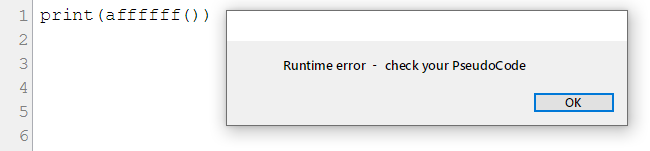
\includegraphics[width=\textwidth]{pseudocodeuk_runtime_err}
	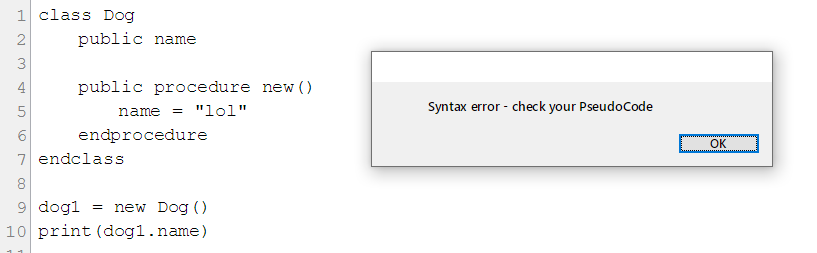
\includegraphics[width=\textwidth]{pseudocodeuk_syntax_err}
	\caption{Screenshots of the error messages provided by PseudoCode
	Interpreter}
	\label{fig:pseudocodeuk_errors}
\end{figure}

\subsubsection{On LLVM}

LLVM has been mentioned multiple times in this section. It is ``a collection of
modular and reusable compiler and tool-chain technologies'' as described by its
website. One of the feature it provides is an intermediate representation (IR)
known as LLVM IR. Many compilers including the rust compiler, the
implementation language, compile the source code given to them to LLVM IR and
then use LLVM to compile this intermediate representation down to machine code.

LLVM will optimise the code and can then compile into many different types of
machine code, it supports a dozen architectures/instruction sets. This allows
those writing compilers to focus on their language rather than having to
implement a back-end to their compiler for every instruction set they want to
support.

We will not be using LLVM as part of this project because it would introduce a
large amount of complexity and unfortunately the documentation for LLVM is
quite sparse.

\subsection{Essential Features}

In of itself, the project is quite self contained and there aren't many
features apart from the core itself: implement a language.

It is possible however to separate the core of the language into different
section; for example, the GCSE features and the A Level (Object-oriented
programming) features can be separated. Considering implementing
object-oriented features is more complex this will allow to have a working
language regardless of how the implementation of other features goes.

Other features which we are unlikely to be able to implement but may be done as
a bonus in order to turn this implementation into a more usable language is
tooling. Here is a list of tooling we could implement although it is quite
unlikely this stage is reached.

\subsubsection{Syntax highlighting}

In order to support syntax highlighting, code editors support various ways to
define syntax, some use tree-sitter such as Atom, or Neovim with tree-sitter
support. Others use their own method of specifying the syntax. Lastly, some
editors use the specification of other editors.

As such implementing syntax highlighting would be a lot of work, as every
editor we plan on supporting would require code to be written for.

Syntax highlighting makes code easier to read as the structure is clearly
separated and keywords, variables names and function definitions stand out from
the rest of the code.

\begin{listing}
	\centering
	\begin{minipage}{.5\textwidth}
		\centering
		\begin{minted}{rust}
fn main() {
    println!("Hello, World!");
}
		\end{minted}
	\end{minipage}%
	\begin{minipage}{.5\textwidth}
		\centering
		\begin{minted}{text}
fn main() {
    println!("Hello, World!");
}
		\end{minted}
	\end{minipage}

	\caption{Side-by-side comparison of syntax highlighted and non-syntax
	highlighted code}
\end{listing}

\subsubsection{Playground}

Many modern programming languages have a `playground', a website on which
people can test out the language without having to install any software. For
example the go programming language and rust have one\cite{rustPlayground,
goPlayground}.

This would allow users to test out or even run programs easily which would
lower the barrier to entry, something that is necessary when the target
audience contains students.

Considering the nature of the language, which will be used to test out simple
pieces of code rather than running production-grade services, there is no
necessity for the users to install the software.

\subsubsection{Language Server}

Introduced in 2016 by Microsoft, the language server protocol is a protocol
used by editors to communicate with software that will indicate to the editor
what diagnostics to display to the user. It allows a single program to be
written for each language, as long as the editor supports the protocol, instead
of a plugin being written for every editor and every language out there.

This means that we could write a language server for the OCR reference language
which would add support for the language in all major editors, instead of
having to support each editor individually, minimising bugs and improving the
quality of diagnostics.

\subsubsection{Additional language syntax}

In addition to the language as defined in specification documents, we could add
additional features and syntax. A feature could be to support other pseudocode
languages such as the one used by other exam boards like \textcite{aqaCS} or
\textcite{wjecCS}, this would allow students taking exams from these exam
boards to benefit from this project as well.

We could also add support for features that would make the language more
productive such as a foreign function interface (FFI) with C, which would allow
to call C code and make use of the wide array of libraries already written in
C. FFI support with C is primordial in the success of a language in particular
a high level language like this one because it allows to perform low level
operations and make use of the thousands of libraries that have been written
and C and would simply be impossible to rewrite in another language due to the
amount of work it would require.

An example of C library that would be useful to have within the language is
\citetitle{sqlite}. This SQL database is used by most schools to teach the
database section of the A level course and as such being able to use it within
the programming language would be highly beneficial. \Citetitle{sqlite} being
made up of more than 100,000 lines of code would be impractical to rewrite in
the language and any attempt would result in a much lower code quality.

An alternative to FFI would be to implement interfaces within the interpreter
however this would require the interpreter to be updated for every library that
needs to be supported and as such is impractical.

\subsection{Limitations}

% TODO: students will probably still need to learn another language alongside

A limitation of this solution which we propose is that although this language
will be usable as a general purpose language, students will likely benefit from
also learning another language that is more widely used and is supported by
more libraries. Learning another language will allow students to have a better
grasp of the concept of programming languages and will allow them to understand
and try out the different programming paradigm and language features, something
that is assessed at A Level. Lastly, students who decide to pursue their
studies in computer science will undoubtedly need to learn multiple programming
languages and so we believe that there is little to gain by learning only a
single one. This means that using this implementation in order to avoid
learning two languages is not necessarily beneficial and is probably
detrimental to students for anything greater than short-term time saving, it is
not something we would recommend to students.

Although the language will allow markers to be more lenient when marking code
written by candidates in exams it will not make the marking easier as it will
still be necessary for other syntaxes used by students to be marked correctly
and additionally it will take additional time for the programs written by
students to be transcribed in a digital format so that it can be executed using
the interpreter.

Another limitation of this solution is that the OCR Exam Reference Language is
a language designed to be as neutral as possible and has as its only intended
purpose to represent simple algorithms for exams. As a result, the language is
very limited and cannot be used for much without extensions that add features
to it. This makes it in combination with its non-existent use unsuitable for
building any complex system above a few hundreds lines of code.

One of the most important features of a language is its community: it allows to
have easily available libraries to make development faster without having to
rewrite code that has already been written before. By using a niche language
like this one, a developer is giving up on all the libraries that can make
their life easier. The language doesn't feature a module system to separate
code into multiple files and would allow code to be separated into libraries
for use by others which means that even with a larger user base, it would be
unlikely that the problem described is ever solved. A solution could be to add
a module extension to the language, however, we do not believe that making the
language popular and usable to write business applications is within our aim
and as such will not implement such a feature.

% TODO: reference the design section here

Lastly, another important part of the user experience when it comes to using a
language is tooling. Tooling improves development time and reduces the learning
curve of a language. Although we hope to have syntax highlighting through
tree-sitter (see Design section) and possibly a language server \cite{lsp}, the
tooling will be greatly reduced compared to other languages which means that
the development experience will be less enjoyable and more difficult, leading
to users not being able to write high quality code, and choosing other
languages in favour of this one.

For languages to be successful and as such useful to know, they need a
disrupting feature or another compelling reason to use it. With the language
developed as part of this project, the compelling reason to use it, is related
to exams (whether that be to prepare for them, or to make them) but there are
no other reasons than that and as such it will not be useful to know the
language beyond the reasons just stated which means some users may not find it
worth it to learn and use this project.

\subsection{Hardware and Software requirements}

The language needs to be widely available (as most programming languages are)
and as a result needs to have the least amounts of requirements as possible.
Due to the implementation of the language being in the form of an interpreter
and there being no low level constructs defined (within the OCR spec), the
language doesn't require to run without an operating system (This would be a
requirement if firmwares, operating system and other low level software was
written using the language). As a result a standard operating system will be
required.

The operating systems that will be primarily supported are Linux, MacOS and
Windows (in that order) however the interpreter will be written in a cross
platform fashion (by using libraries to abstract platform specific code) such
that it is most likely going to work on any other modern operating system such
as the BSDs.

If a playground is offered, a browser implementing the standard browser
specifications should be required, alongside a working internet connection. The
playground version will not have restrictions on the host operating system. The
web version could be implemented using web assembly in which case a modern
browser supporting WebAssembly will be required. If the web version is
implemented by running the interpreter on a server, the server will require one
of the operating systems aforementioned.

There are no hardware requirements other than dependencies on already mentioned
software requirements. Interpreters are not resource intensive programs and can
even execute on most low power micro controllers\cite{micropython}.

Because we will be using rust to implement the project, we will be limited by
the platforms rust support, which is to say we will not be limited as rust
supports all major platforms\cite{rustPlatformSupport}.

\subsection{Success Criteria}

For the main part of this project, the interpreter that will execute programs
written in the OCR reference language, the success criteria would be that the
interpreter works. This means that when given valid code, it should be able to
execute it and return to the user what is expected.

However, this is quite a general definition and within the interpreter they may
be some features of the language that works while others don't and as such we
need to break down this larger success criteria into smaller sub-parts. The
sub-parts can be defined in terms of features of the language.

Following is a list of the features that should be tested to measure how
successful the project was. The list is derived from the pseudocode guide in
\citetitle{h446}:

\begin{enumerate}
	\item Being able to read a file
	\item Working sequential instructions
	\item Comments
	\item Outputting to screen
	\item Variables
	\item Iteration---Count Controlled
	\item Selection
	\item Logical Operators
	\item Iteration---Condition Controlled
	\item String Handling
	\item Subroutines
	\item Subroutines---Passing values by value or by reference
	\item Arrays
	\item Reading from files
	\item Writing to files
	\item Objects---Attributes
	\item Objects---Methods
	\item Object---Access level
	\item Object---Constructors
	\item Object---Inheritance
\end{enumerate}

In order to make the success criteria more objective, it would be preferable if
these features can be tested as much as possible in an automatic way to remove
bias. This would also make the testing more efficient.

\subsubsection{Success criteria for optional features}

To consider syntax highlighting, to be complete, for the editors for which syntax
highlighting is implemented, keywords, and structures that make up the language
should be highlighted accordingly. The syntax defined for the syntax
highlighting should have no bugs such that the different elements of the code
are highlighted in a coherent way. If the highlighting is not coherent it would
be confusing for the user and would result in reduced productivity.

For the playground, the language should be usable with as much of the features
of the language being usable from the playground. Some features will be more
difficult to implement as an inherent result of the platform. For example
reading and writing to files on the web makes little to no sense and it is
perfectly acceptable if this is not achieved. However, it can be possible to
implement it for example by having a virtual file system to which users can
upload files.

The success criteria for the language server would involve having produced a
language server that is usable by most editors in particular those of interest
for us are Neovim and VS code. If the language server works for both of these
editors it can be considered that it is stable enough and should work for most
others. The language server should be able to display appropriate errors to the
user and assist them in their development.

For all additional language features, the success criteria would be that the
feature is functional and works as intended.

\section{Design of the interpreter}
\label{sec:design_int}

\subsection{Type of programming language implementation}

There are 2 main ways to be able to write language: as an interpreter or as a
compiler. Additionally there are also different flavours of just-in-time (JIT)
compilers.

Interpreters work by directly executing the instructions indicated by the
program. For example, if in the programming language, there is a print
instruction, the interpreter will print the text corresponding to the operand
of that print instruction.

Compilers work by translating the source code into another type of code.
Generally compilers compile code down to a lower level representation of the
code but sometimes they transform the code into a language of a similar level
of abstraction from the source language, for example to JavaScript. These types
of compilers are usually called ``transpilers''. For example the
\citetitle{nim} compiler compiles Nim source code down to JavaScript or C.
Compilers are generally more difficult to implement as they have greater
complexity and the lower the level of abstraction the target language is the
greater the complexity of the compiler generally is. Ultimately some compilers
compile to machine code, code that can be directly executed on the CPU.

In addition to compilers and interpreters, there are just-in-time compilers
which compile code to machine code as it is executed, often just-in-time
compilers are a hybrid of a compiler and an interpreter, such that code is
interpreted at first and then compiled to obtain a greater performance. This is
how the JavaScript engines that run in major browsers (V8, SpiderMonkey and
JavaScriptCore, for Chromium, Firefox and Safari respectively) are implemented.

For our programming language, we have decided to opt for an interpreter design
due to the language's dynamic nature, the lesser complexity of implementation
of interpreters and the much greater cross-platform compatibility.

\subsection{Language of implementation}

The implementation language will be rust because it is a language the author is
familiar with and because it is a high performance language as it compiles to
machine code. This is very important when writing an interpreter because it
will allow to have acceptable performance. Writing an interpreter in an
interpreted language would accumulate overhead and result in bad performance.

Additionally, Rust supports a very wide array of operating systems and CPU
architectures/instruction set. This is particularly important as we plan on
building a playground which will execute code on the client side using
WebAssembly (wasm)\cite{wasm}, a web standard which defines a bytecode that can
be executed by browsers. As of now very few languages have good support for
WebAssembly, but it is generally considered that rust has be the best support,
even though, it is still not straight forward to use it.

\subsection{Parsing}

Now that we have made the high-level design decisions, we will look at the
implementation of the interpreter itself. Figure
\ref{fig:interpreting_flowchart} shows the major steps involved in the
interpretation of a program.

\begin{figure}
	\centering
	\begin{tikzpicture}[node distance=2cm]
		\node (start) [terminal] {Start};
		\node (parsing) [process, below of=start] {Parsing};
		\node (interpreting) [process, below of=parsing] {Interpreting};
		\node (end) [terminal, below of=interpreting] {End};
		\draw [flowchartarrow] (start) -- (parsing);
		\draw [flowchartarrow] (parsing) -- (interpreting);
		\draw [flowchartarrow] (interpreting) -- (end);
	\end{tikzpicture}
	\caption{The major steps carried out by an interpreter}
	\label{fig:interpreting_flowchart}
\end{figure}

The first step of interpreting any kind of code is parsing. This stage involves
converting text into a structured object which can then be used for other
purposes, most importantly evaluating/interpreting the object to execute the
code it represents. The object generated is known as an abstract syntax tree
(AST) and represents the program to be executed as a tree data structure.

There are numerous methods of writing a parser, they generally fall under two
wide categories, manual parsing, or parsing using parser generators. Parser
generators are programs to which which output a parser given a language
grammar, a definition of the syntax of a language and its structure. The parser
is then capable of parsing the input. On the other hand, when writing parsers
manually instead of having the parser generated for us based on a language
grammar, we write ourselves the code that would parse the input.

At first we were hoping to use \citetitle{treesitter} as our parsing system
because it would give us syntax highlighting inside of editors without having
to write a regex based grammar or another parser. Being able to re-use the
parser used for the language as well as for syntax highlighting increases the
robustness of the software, because a single shared implementation is used and
bugs that are found are fixed for both, and both stay consistent with each
other. Additionally using a parser generator is generally less error prone as
the parser generator is unlikely to produce invalid code and less time
consuming as only a grammar has to be written instead of a parser, something
much more complex.

However in the end we decided to write our own parser because writing
tree-sitter grammars is not an easy task and is described as having ``a
difficult learning curve''\cite{ts_creating_parsers} and tree-sitter loads
language grammars as shared libraries which would have been difficult to use
within the playground from web assembly as the grammar itself would be a web
assembly module in addition to the interpreter which would also be a
WebAssembly module. Lastly, writing a parser is generally not considered to be
the most complex task of writing an interpreter and writing our own gives us
much more flexibility.

This is why we have decided to use a different method for parsing the code. We
settled on using parser combinators with the help of the parser combinator
framework \citetitle{nom}. This library was chosen because it is the most widely
used parsing framework for rust (our implementation language) and the author
has experience having used it while going through \textcite{eopl} to prepare
for this project.

Another advantage of using parser combinators is that they allow to perform
complex transformations during the parsing. For example, it is possible to
transform a switch statement into if statements and else-if statements into
if and else statements during the parsing instead of in a different pass, this
allows to reduce the complexity of subsequent passes at the cost of increasing
the complexity of the parser. Ultimately, we only perform a single pass before
interpreting the abstract syntax tree: parsing, nothing more. Unlike many
interpreters were the source code has to be tokenized before and once the
source code has been parsed it needs to be transformed again into a form that
can be used for interpretation.

This advantage comes directly from another major advantage of using a parser
combinator based method: flexibility. The other major method would be to use a
parser generator library, the method recommended by \textcite{eopl}, such as
\textcite{bison}. The downside of this is that the program will have to be
built upon the structure of the parser and will be limited by it.

\subsubsection{On parser combinators}

Parser combinators are an implementation of the recursive descent algorithm,
they work by chaining functions to parse more complex structures. The recursive
descent algorithm attempts to parse different elements of the input and then
backtracks when it fails, until it eventually succeeds or fail, in which case
it fails to parse the input. This can happen if the input is malformed or if
there's a bug in the parser.

\subsubsection{Language Grammar}

Because we are writing our parser using a parser combinator design, we will
have to define a function for every element we want to parse. In order to do
this we first have to define every element that makes up our language or
otherwise we risk forgetting some elements.

This definition of the structures in a language can be represented in many
different ways, but in our case we will define it as a language grammar. A
language grammar defines all the possible different statements and expressions
found in the language to simplify writing the parser. If we used a method using
parser generators we would normally have given our grammar to the parser
generator so it then generates the parser. In our case, because we are writing
the parser ourselves we are only doing it in order to more easily keep track of
everything that has to be implemented.

The language grammar we define is informal as it is only meant to be read by
humans, unlike one that is used with a parser generator. Each definition is
made up of the left-hand-side and the right-hand-side separated by ``::=''.
The left-hand-side represents the element that is being defined. When an
element is defined multiple times, we are defining the different forms this
element can have. For example a statement can an assignment of a variable but
it can also be a for loop.

The root of the tree is the Program element and from where the parsing starts
with. Comments are not defined in this grammar but they are any text prefixed
by two forward slashes: ``//''.

It can be found at listing \ref{lst:grammar}.

For every element of the of the grammar, and for every variant of every
element, a function will be defined that parses that element using other
functions.

\begin{listing}
	\noindent
	Statement ::= \texttt{global} Identifier \texttt{=} Expression\\
	Statement ::= Identifier \texttt{=} Expression\\
	Statement ::= \texttt{array} Identifier\texttt{[}\{Expression\}\textsuperscript{+(\texttt{,})}\texttt{]}\\
	Statement ::= Expression\\
	Statement ::= \texttt{for} Identifier \texttt{=} Expression \texttt{to} Expression List-of-Statements \texttt{next} Identifier\\
	Statement ::= \texttt{while} Expression List-of-Statements \texttt{endwhile}\\
	Statement ::= \texttt{do} List-of-Statements \texttt{until} Expression\\

	\noindent
	Statement ::= \texttt{if} Expression \texttt{then} List-of-Statements \{\texttt{elseif} Expression \texttt{then} List-of-Statements\}\textsuperscript{*} \{\texttt{else} List-of-Statements\}\textsuperscript{?} \texttt{endif}\\
	Statement ::= \texttt{switch} Expression\texttt{:} \{\texttt{case} Expression\texttt{:} List-of-Statements\}\textsuperscript{*} \{\texttt{default:} List-of-Statements\}\textsuperscript{?} \texttt{endswitch}\\

	\noindent
	Statement ::= \texttt{function} Identifer\texttt{(}\{Identifier\{:byVal | :byRef\}\}\textsuperscript{*(\texttt{,})}\texttt{)} List-of-Statements \texttt{endfunction}\\
	Statement ::= \texttt{procedure} Identifer\texttt{(}\{Identifier\{:byVal | :byRef\}\}\textsuperscript{*(\texttt{,})}\texttt{)} List-of-Statements \texttt{endprocedure}\\
	Statement ::= \texttt{return} Expression\\

	\noindent
	List-of-Statements ::= ()\\
	List-of-Statements ::= (Statement . List-of-Statements)\\

	\noindent
	Expression ::= Constant\\
	Expression ::= Identifer\texttt{(}\{Expression\}\textsuperscript{*(\texttt{,})}\texttt{)}\\
	Expression ::= Identifier\texttt{.}Field\\
	Expression ::= Identifier\texttt{.}Method\texttt{(}\{Expression\}\textsuperscript{*(\texttt{,})}\texttt{)}\\

	\noindent
	Expression ::= Expression \texttt{AND} Expression\\
	Expression ::= Expression \texttt{OR} Expression\\
	Expression ::= \texttt{NOT} Expression\\

	\noindent
	Expression ::= Expression \texttt{==} Expression\\
	Expression ::= Expression \texttt{!=} Expression\\
	Expression ::= Expression \texttt{\textless{}} Expression\\
	Expression ::= Expression \texttt{\textless=} Expression\\
	Expression ::= Expression \texttt{\textgreater{}} Expression\\
	Expression ::= Expression \texttt{\textgreater=} Expression\\

	\noindent
	Expression ::= Expression \texttt{+} Expression\\
	Expression ::= Expression \texttt{-} Expression\\
	Expression ::= Expression \texttt{*} Expression\\
	Expression ::= Expression \texttt{/} Expression\\
	Expression ::= Expression \texttt{MOD} Expression\\
	Expression ::= Expression \texttt{DIV} Expression\\
	Expression ::= Expression \texttt{\textasciicircum{}} Expression\\

	\noindent
	Program ::= List-of-Statements
	\caption{The grammar for our language}
	\label{lst:grammar}
\end{listing}

Using this grammar we are able to declare classes that define possible nodes on
the tree. In our particular implementation, we will use Rust's \texttt{enum}
feature which allows to define objects that can be one of many variant. In our
implementation we will have two types of elements: Statements and Expressions.
Our \texttt{Expression} enum will have all the different types of expression
and the \texttt{Statement} enum will have all the different types of statements
as defined in listing \ref{lst:grammar}. Statements can be put together into a
list known as a list of statements, this represents blocks of codes that can be
found in this language.

The major differences between expression and statements is that expressions
evaluate to a value whereas statements do not evaluate to anything, they only
perform an action. This distinction of evaluating and only performing an
operation also exists in the language in the form of the co-existence of
procedures and functions where in other languages they would be one. In our
implementation we treat them as one with the only difference between the two
being that functions when called return a value whereas statements return
nothing, or to be more precise they return a value indicating that no value was
returned.

Ultimately, because statements can also be return statements that return
values, lists of statements are effectively expressions and so are all
statements that contain a list of expression that they could execute or not.

\subsubsection{Implementation details}

Parser combinators can cause issues when multiple parsers succeed at parsing a
given input. An example of this is numbers, a parser for floating point numbers
will generally succeed at parsing integers and vice versa. In our
implementation we have decided to use the algorithm presented in
\autoref{fig:number_parse_alg}. It allows to parse float and integer
literals\footnote{In programming languages,
\href{https://en.wikipedia.org/wiki/Literal_(computer_programming)}{literals}
are fixed values that are represented directly in the code} in the way the user
expects it to happen. The way it works is that if either parser fails it
returns the result of the other parser or otherwise returns the result of the
parser that consumed the post input. Note that our parser combinators return a
\texttt{Result} type which is why it is fine the return the result of the
integer parser even if it failed, this just means the result will propagate
down without affecting the ultimate result.

\begin{figure}
	\centering
	\begin{tikzpicture}
		\node (start) [terminal] {Parse number};
		\node (parse_int) [process, below = 0.7cm of start] {Attempt to parse integer};
		\node (parse_float) [process, below = 0.7cm of parse_int] {Attempt to parse float};
		\node (int_err) [decision, below = 0.7cm of parse_float] {Did integer parsing
		succeed?};
		\node (return_float) [terminal, right of = int_err, node distance=5cm] {Return float};
		\node (float_err) [decision, below = 0.7cm of int_err] {Did float
		parsing succeed?};
		\node (return_int) [terminal, right of = float_err, node distance=5cm] {Return integer};
		\node (which_longest) [decision, below = 0.7cm of float_err] {Did
		integer parsing consume more input than float parsing?};
		\node (return_float2) [terminal, right of = which_longest, node
		distance=5cm] {Return float};
		\node (return_int2) [terminal, below = 0.7cm of which_longest] {Return integer};
		\draw [flowchartarrow] (start) -- (parse_int);
		\draw [flowchartarrow] (parse_int) -- (parse_float);
		\draw [flowchartarrow] (parse_float) -- (int_err);
		\draw [flowchartarrow] (int_err) -- node[anchor=south] {no} (return_float);
		\draw [flowchartarrow] (int_err) -- node[anchor=east] {yes} (float_err);
		\draw [flowchartarrow] (float_err) -- node[anchor=south] {no} (return_int);
		\draw [flowchartarrow] (float_err) -- node[anchor=east] {yes} (which_longest);
		\draw [flowchartarrow] (which_longest) -- node[anchor=south] {no} (return_float2);
		\draw [flowchartarrow] (which_longest) -- node[anchor=east] {yes} (return_int2);
	\end{tikzpicture}
	\caption{Flowchart of the process involved in parsing a number}
	\label{fig:number_parse_alg}
\end{figure}

Many decisions had to be taken in regards to the design of the language itself
because it was never strictly defined in the exam specifications from OCR. For
example the format of identifiers (class, function and variable names) is not
defined. So we decided to have a design similar to most languages (such as
python and rust): identifiers can be made of letters and digits, as well as
underscores however they cannot start with a digit\footnote{These are the same
rules as for python:
\url{https://docs.python.org/3/reference/lexical_analysis.html\#identifiers}}.
The reason most languages do this and we have decided to follow their decision
is because having an identifier start with a digit makes parsing more difficult
as a integer literal parser could succeed when what is being parsed is not a
number but rather an identifier. Identifiers also cannot contain dashes as
these are used for the minus sign.

The last two design decisions have been made due to parsers not being mutually
successful (i.e. multiple parsers can succeed for a given input).

Another design decision we had to take and for which we ultimately settled on a
design inspired by python was division and what value type they would return.
In the end we settled for a design similar to python in which any kind of non
whole number division returns a floating point number.

Another difficult issue to tackle was how we were going to implement
exponentiation. This is a very complex operation which on one hand people
generally wish to return an integer if possible but on the other hand requires
to return a floating point value if need be. We settled for a design inspired
from python which can be found in listing \ref{lst:power_alg}.

\begin{listing}
	\begin{minted}{text}
function exponentiation(base, exponent)
	if is_integer(base) then
		if is_integer(exponent) then
			if exponent >= 0 then
				return integer_exponentiation(base, exponent)
			else
				// if the exponent is negative
				return float_exponentiation(base, exponent)
			endif
		else
			return float_exponentiation(base, exponent)
		endif
	else
		return float_exponentiation(base, exponent)
	endif
endfunction
	\end{minted}
	\caption[Pseudocode describing the algorithm for exponentiation]{Pseudocode
	describing the algorithm for exponentiation\protect\footnotemark}
	\label{lst:power_alg}
\end{listing}

\footnotetext{In reality the algorithm is more complex in order to have
performance improvements when the exponent is an integer but a float result is
wanted.}

\subsection{Interpreting}

To interpret a program we will simply go over the structure of it executing its
statements one-by-one.

In order to deal with state: classes, functions, and variables defined
throughout our program, we will have a \textbf{\texttt{Context}} object that
holds all the state of our program. It will be made of a hash table from
function names to function objects, a hash table of class names to class
objects and lastly, an environment. The environment is a list\footnote{in this
section ``list'' is used as a generic term, however implementation-wise we use
rust's \citetitle{vec} type.} of hash tables mapping from variable names to
values.

Each hash table in the list represents a different stack frame. The first
element is the global scope and each time a function is called a new element is
added.

Because our language supports references, there are multiple ways of storing
values. One of them is to have a list containing the values and then store in
the environment references to the index of the elements in the list. One
problem of this approach is that it doesn't garbage collect elements once they
are unused.

This is why we have decided to use the rust language's built-in types to deal
with garbage collection. Each denoted value is a reference counted value, such
that once there are no references to the value it is dropped and memory is
freed.

To simplify the implementation, values are implemented entirely in rust and use
overloading (using the traits in rust) to make the use of values within the
interpreter easier. This can have downsides as it abstracts away the values
however it means that when writing the interpreter less time is wasted.

Objects are stored as a list of values, each value representing a field in the
object. Overloading works using a method similar to lexical
addressing\footnote{Lexical addressing is a method in which textual variables
are converted into numbers, this allows for improved performance because
variables are now just indices in a list, something that has an order O(1)
lookup}, in that attribute names are converted into indices within the object.

However we do not use lexical addressing anywhere else, this means that strings
are stored in the class objects (that part of the context) and hash tables are
used for everything instead of lists. The reason for this is we have found it
difficult to implement whilst following other resources as preparation for this
project.

It would also have been a possibility to implement functions as values as is
common in most programming languages however we preferred to not implement
functions as values as when we were going through \citetitle{eopl} whilst
preparing to write this interpreter we found great difficulty in implementing
mutually recursive functions, something that is not a problem when functions
are not values but rather an item in a \texttt{HashMap}\footnote{Rust's hash
table present in the standard library}.

\subsection{Testing}

Testing is very important in maintaining stable software that behaves as
intended. It allows to define the behaviour of our software and prevent
regressions from occurring. For this project we will be using automated testing
to test our software because it will allow to consistently tests anything in a
much faster and objective way. It will allow to test hundreds of components in
mere seconds which will be a great productivity boost. By making the friction
of testing so much smaller it also means we will be testing much more often
leading to mistakes being found faster. Lastly, it will allow us to use a
software development process known as test-driven development in which tests
are written before the code it tests is written. Using this approach will
improve productivity because it gives a clear goal during the development
process and also prevents the test to be built around the behaviour of the
already written code rather than the other way around which would mean the
tests are bias and may not be suitable.

Additionally because we will be building the parser first, there will be no
convenient way for a human to test the parser and writing tests would allow to
test the parser, without having to write an interface for a human tester (or
any other way that involves a human in the process of testing the parser). Once
the interpreter is developed, it is then possible for a human to test the
program manually as they can see the result of the program they run.

In order to test the software and validate the success criteria in an objective
way, a testing script \texttt{neasuccess} will be written before the
implementation has started to be written. This test script will run the
implementation with different inputs and verify that the output is the one
expected.

The success test script will be modular and be able to support many different
tests. It will work in the following way: In the \texttt{tests} directory,
there will be files with the extension \texttt{.input} and \texttt{.output}.
The success test script will run the interpreter with as input the content of
the \texttt{.input} files and check if the output is the same as the file with
the same basename but as extension \texttt{.output} file. In order to test the
parser, we will also have \texttt{.ast} files containing a representation of
the AST to which to parser can compare the result to.

An argument can be given to the success test script to only use the tests with
the basename given.

In table \ref{tbl:success_criteria} the success criteria defined in the
analysis are listed alongside the way they will be able to be tested using the
\texttt{neasuccess} script and the test data. The test data will be displayed
with the input on the top/left and the expected output on the bottom/right with
a grey background. It is highly likely that some of the features in the success
criteria will be implemented together rather than sequentially.

The test data given to test for the success criteria are deliberately very
simple so that they only test the success criteria in question, however in
development, we will use much more complex tests when appropriate to test the
entirety of the interpreter at once.

\begin{table}
    \begin{adjustbox}{center}
        \begin{tabular}{|l|l|l|}
            \hline
			Criteria & How to evidence & Code \\
            \hline
            Being able to read a file & Run the interpreter with a file as input & \\
            \hline
			Working sequential instructions & Run \texttt{./neasuccess seq} & Listing \ref{lst:design_seq} \\
            \hline
			Comments & Run \texttt{./neasuccess comments} & Listing \ref{lst:design_comment} \\
            \hline
			Outputting to screen & Run \texttt{./neasuccess print} & Listing \ref{lst:design_print} \\
            \hline
			Variables & Run \texttt{./neasuccess variables} & Listing \ref{lst:design_variables} \\
            \hline
            Iteration---Count Controlled & Run \texttt{./neasuccess forloop} & Listing \ref{lst:design_for_loop} \\
            \hline
			Selection & Run \texttt{./neasuccess selection} & Listing \ref{lst:design_string_handling} \\
            \hline
			Logical Operators & Run \texttt{./neasuccess logic} & Listing \ref{lst:logical_operators2} \\
            \hline
            Iteration---Condition Controlled & Run \texttt{./neasuccess whileloop} & Listing \ref{lst:design_while_loop} \\
            \hline
			String Handling & Run \texttt{./neasuccess strings} & Listing \ref{lst:design_string_handling} \\
            \hline
			Subroutines & Run \texttt{./neasuccess subroutines} & Listing \ref{lst:design_subroutine_run} \\
            \hline
            Subroutines---Passing values by value or by reference & Run \texttt{./neasuccess byvalue\_byref} & Listing \ref{lst:design_byref} \\
            \hline
			Arrays & Run \texttt{./neasuccess arrays} & Listing \ref{lst:design_subroutine_run} \\
            \hline
			Reading from files & Run \texttt{./neasuccess readfile} & Listing \ref{lst:design_read_from_file} \\
            \hline
			Writing to files & Run \texttt{./neasuccess writefile} & Listing \ref{lst:copy_file} \\
            \hline
			Objects---Attributes & Run \texttt{./neasuccess attributes} & Listing \ref{lst:oop_attributes} \\
            \hline
			Objects---Methods & Run \texttt{./neasuccess methods} & Listing \ref{lst:oop_inheritance_and_methods} \\
            \hline
			Object---Access level & Run \texttt{./neasuccess access} & Listing \ref{lst:access_level} \\
            \hline
			Object---Constructors & Run \texttt{./neasuccess constructors} &
			Listing \ref{lst:oop_attributes} and
			\ref{lst:oop_inheritance_and_methods} \\
            \hline
			Object---Inheritance & Run \texttt{./neasuccess inheritance} & Listing \ref{lst:oop_inheritance_and_methods} \\
            \hline
        \end{tabular}
    \end{adjustbox}
    \caption{Success Criteria}
	\label{tbl:success_criteria}
\end{table}

\begin{listing}
	\inputminted{text}{./prog/prog/test_data/design_seq.input}
	\inputmintedgrey{text}{./prog/prog/test_data/design_seq.output}
	\caption{Test data for executing sequential instructions}
	\label{lst:design_seq}
\end{listing}

\begin{listing}
	\inputminted{text}{./prog/prog/test_data/comment1.input}
	\inputmintedgrey{text}{./prog/prog/test_data/comment1.output}
	\caption{Test data with comment}
	\label{lst:design_comment}
\end{listing}

\begin{listing}
	\begin{minipage}{.5\textwidth}
		\inputminted{text}{./prog/prog/test_data/print.input}%
	\end{minipage}%
	\begin{minipage}{.5\textwidth}
		\inputmintedgrey{text}{./prog/prog/test_data/print.output}
	\end{minipage}
	\caption{Test data for printing}
	\label{lst:design_print}
\end{listing}

\begin{listing}
	\inputminted{text}{./prog/prog/test_data/design_variables.input}
	\inputmintedgrey{text}{./prog/prog/test_data/design_variables.output}
	\caption{Test data for variables}
	\label{lst:design_variables}
\end{listing}

\begin{listing}
	\inputminted{text}{./prog/prog/test_data/for_loop1.input}
	\inputmintedgrey{text}{./prog/prog/test_data/for_loop1.output}
	\caption{Test data for for loops}
	\label{lst:design_for_loop}
\end{listing}

\begin{listing}
	\inputminted{text}{./prog/prog/test_data/logical_operators2.input}
	\inputmintedgrey{text}{./prog/prog/test_data/logical_operators2.output}
	\caption{Test data for logical operators}
	\label{lst:logical_operators2}
\end{listing}

\begin{listing}
	\inputminted{text}{./prog/prog/test_data/design_while.input}
	\inputmintedgrey{text}{./prog/prog/test_data/design_while.output}
	\caption{Test data for while loops}
	\label{lst:design_while_loop}
\end{listing}

\begin{listing}
	\inputminted{text}{./prog/prog/test_data/design_string_handling.input}
	\inputmintedgrey{text}{./prog/prog/test_data/design_string_handling.output}
	\caption{Test data for string handling and selection}
	\label{lst:design_string_handling}
\end{listing}

\begin{listing}
	\inputminted{text}{./prog/prog/test_data/design_byref.input}
	\inputmintedgrey{text}{./prog/prog/test_data/design_byref.output}
	\caption{Test data for passing data by reference and by value}
	\label{lst:design_byref}
\end{listing}

\begin{listing}
	\inputminted{text}{./prog/prog/test_data/design_subroutine_run.input}
	\inputmintedgrey{text}{./prog/prog/test_data/design_subroutine_run.output}
	\caption{Test data for running subroutines and arrays}
	\label{lst:design_subroutine_run}
\end{listing}

\begin{listing}
	\inputminted{text}{./prog/prog/test_data/design_read_from_file.input}
	\inputmintedgrey{text}{./prog/prog/test_data/design_read_from_file.output}
	\caption{Test data to check whether it is possible to read from files}
	\label{lst:design_read_from_file}
\end{listing}

\begin{listing}
	\inputminted{text}{./prog/prog/test_data/copy_file.input}
	\inputmintedgrey{text}{./prog/prog/test_data/copy_file.output}
	\caption{Test data for writing to files}
	\label{lst:copy_file}
\end{listing}

\begin{listing}
	\inputminted{text}{./prog/prog/test_data/class3.input}
	\inputmintedgrey{text}{./prog/prog/test_data/class3.output}
	\caption{Test data for object attributes}
	\label{lst:oop_attributes}
\end{listing}

\begin{listing}
	\inputminted{text}{./prog/prog/test_data/class4.input}
	\inputmintedgrey{text}{./prog/prog/test_data/class4.output}
	\caption{Test data demonstrating method calls and inheritance}
	\label{lst:oop_inheritance_and_methods}
\end{listing}

\begin{listing}
	\inputminted{text}{./prog/prog/test_data/access_level.input}
	\caption{Test data for testing access level. If the language is implemented correctly, this should fail}
	\label{lst:access_level}
\end{listing}

% TODO (don't forget about ./savedstuff.tex)

\section{Design of the playground}

As briefly mentioned at the beginning of the design of the interpreter, by
having the interpreter written in rust allows us to compile it down to
WebAssembly which means that we can then execute our interpreter in the browser
allowing users to run snippets of code.

A major advantage of using this method to implement a playground is that it
doesn't require a complex back-end, a simple web server suffices as we only
need to serve static files. This means we do not have to deal with scaling and
resource usage and there is no risk of vulnerabilities in the sandbox executing
user code as there is no sandbox and no user code is executed on our servers.

Because we only need to serve static files, it means that we can use one of the
many free services available online that will allow us to serve static files.
In our case we will use GitHub Pages to host the playground for no cost. If the
implementation was similar to that used by go or rust, we would have much
higher cost as we would need to pay for a server to host the playground and in
addition to that would not be able to scale to a larger number of users.

Another advantage of this client-side method is that the application can be
interactive, it can print text to the screen in real time and accept input from
the user, something that is rarely seen in traditional playgrounds because it
only displays the result to the user once the code has finished executing.

Another approach to making a playground interactive is to use WebSockets, such
that whenever the user types something it is sent to the server and whenever
the server prints something it is sent by to the user's browser. This is the
approach used by the interactive shell available on python's homepage visible
in figure \ref{fig:python-playground}.

However this approach has some downsides, first of all it is much slower than
our approach as it has to incur the cost of network latency and having to send
every operation over the network. Secondly it is very complex to implement and
requires having servers that are always on and have to deal with a large amount
of state: each user currently using an iterative session is state to keep
track of.

\begin{figure}
	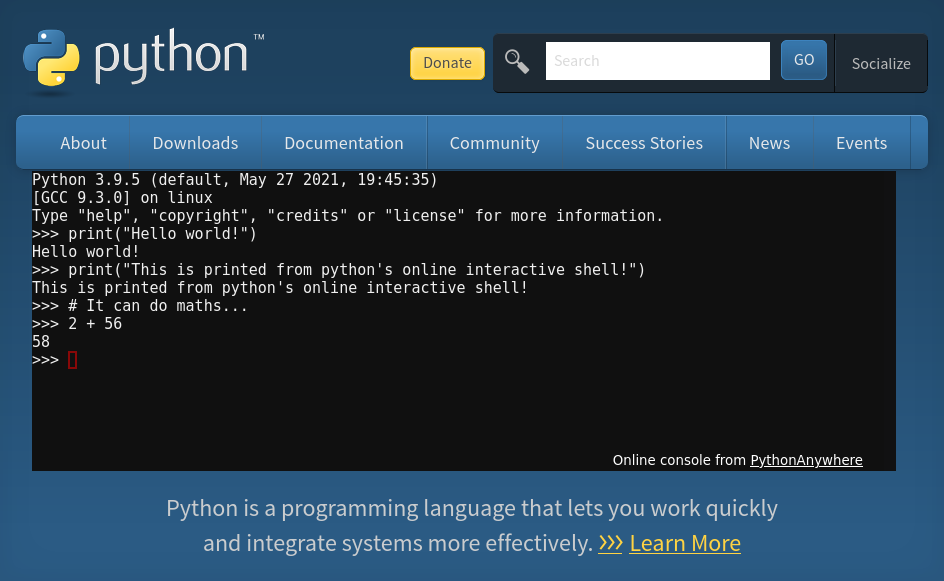
\includegraphics[width=\textwidth]{python-playground}
	\caption{Screenshot of the python online iterative shell}
	\label{fig:python-playground}
\end{figure}

\begin{figure}
	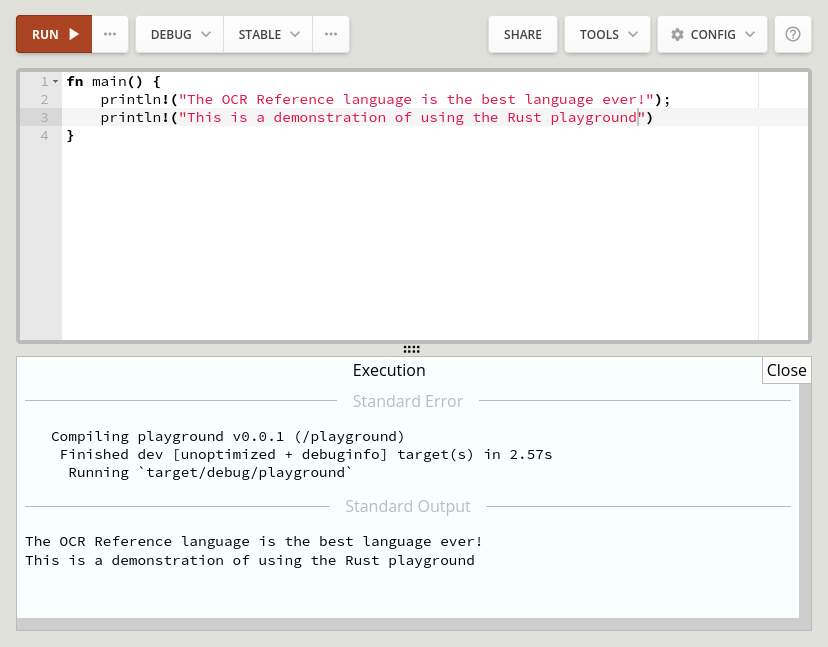
\includegraphics[width=\textwidth]{rust-playground}
	\caption{Screenshot of rust's official playground}
	\label{fig:rust-playground}
\end{figure}

\subsection{Implementation details}

Figure \ref{fig:playground_flow} shows the major steps executed by the
playground. In order to compile our interpreter to WebAssembly we will have a
second crate\footnote{Crates are the name given to packages in Rust} that has
as dependency our interpreter and will have platform specific code for
WebAssembly. This will include dealing with IO on the web which is much
different than natively, as on the web we are not actually printing to a file
but rather modifying the DOM\footnote{Document Object Model, the structure of
the web page}.

This means that our interpreter when printing won't be able to just print
normally otherwise it would not be possible to support this in WebAssembly,
instead we will make it `Write'\footnote{The `Write' trait is the one that will
be used} to some generic object which will be different based on the platform.
This is similar to polymorphism in other languages, except the polymorphism is
done at compile time rather than runtime which is what allows Rust to be such a
high performance language.

\begin{figure}
	\centering
	\begin{tikzpicture}[node distance=2cm]
		\node (start) [terminal] {Website is loaded};
		\node (load_UI) [process, below of=start] {Load user interface};
		\node (load_int) [process, below of=load_UI] {Load wasm module for interpreter};
		\node (wait_for_input) [io, below of=load_int] {Wait for user to submit code};
		\node (interpret) [process, below of=wait_for_input] {Execute program};
		\node (print) [io, below of=interpret] {Print generated output};
		\node (end) [process, below of=print] {Program finishes executing};
		\node (terminate) [terminal, below of = end] {Browser tab is closed};
		\draw [flowchartarrow] (start) -- (load_UI);
		\draw [flowchartarrow] (load_UI) -- (load_int);
		\draw [flowchartarrow] (load_int) -- (wait_for_input);
		\draw [flowchartarrow] (wait_for_input) -- (interpret);
		\draw [flowchartarrow] (interpret) -- (print);
		\coordinate [right = 0.5cm of print] (temp);
		\coordinate [above = 1cm of interpret.north, above of = temp ] (temp1);
		\draw [flowchartline, sloped] (print.east) -- (temp) -- node
		{\midarrow} (temp1) -| (interpret.north);
		\draw [flowchartarrow] (print) -- (end);
		\draw [flowchartarrow, sloped] (end.south) |- ++(3.4cm,-0.5cm) --
		node {\midarrow} ($(wait_for_input.north) + (3.4cm,0.5cm)$) -| (wait_for_input.north);
		\draw [flowchartarrow] (end) -- (terminate);
	\end{tikzpicture}
	\caption{User flow when they visit the playground}
	\label{fig:playground_flow}
\end{figure}

\subsection{Usability features}

The playground will be separated into two sections, an editor to a side and a
pane with the result of executing the program in another pane. In the editing
pane the user will be able to enter their source code and they can then execute
it or print the abstract syntax tree that was produced after parsing their
code. The ability to print abstract syntax tree is beneficial for students to
understand how parsing works and is useful for the development of the project
itself to debug mistakes in parsing.

\subsection{Testing}

Because this is a user facing application it is more difficult to test it in an
automatic manner. Generally to test such web applications a headless browser is
used however we have decided to leave this section untested as it doesn't have
many features and as such wouldn't be too time consuming to test manually. This
is because most of the features are implemented in the interpreter which is
already tested separately, the playground is just a thin wrapper around the
interpreter adding little functionality.

The list of tests to do manually can be found in table
\ref{tbl:playground_tests}.

\begin{table}
	\begin{adjustbox}{center}
	\begin{tabular}{|l|l|l|}
		\hline
		What is being tested & How to test & Success criteria \\
		\hline
		Printing & \makecell[ll]{Enter a simple program \\ and then run it} & Verify that the
		output is correct \\
		\hline
		\makecell[ll]{Errors when given \\ invalid code} & Enter an invalid program &
		\makecell[ll]{Verify that there is an error \\ message indicating where
		in \\ the program a mistake was found} \\
		\hline
		Inputting & \makecell[ll]{Enter a program that asks \\ for the user to
		input data} &
		Verify that inputting data works \\
		\hline
	\end{tabular}
	\end{adjustbox}
	\caption{Tests to do on the playground}
	\label{tbl:playground_tests}
\end{table}

\section{Development}

In order to make development efficient we have used the version control system
\citetitle{git}. This allows us to create snapshots of our software as we move
along the stages of development and allows us to experiment with features which
we can then roll back or accept into our main branch.

Note: In this section tests are often referenced, they will rarely be listed
here but can be found in the section \nameref{sec:final_project} on page
\pageref{sec:final_project}. Additionally, code is rarely included because it
would make the report way too long and all code written can be found in the
final section. The final project at the end of this document is already more
than 100 pages, to reach these 100 pages of code twice the amount of code had
to be written, which would make this document 300 pages of code, something that
is not possible.

\subsection{Stage \subsecnum}

In the first stage of development we focused only on the parser. Using the
grammar described in design we wrote the \texttt{struct}\footnote{The
equivalent to classes found in low level languages} for the tree and then wrote
a parser for it, making sure to implement all the possible variants.

In the first version, unlike what was ``promised'' in the design section of
this document we did not write a testing tool and so in order to be able to
test source code we wrote our tests in Rust using its builtin testing
framework. The test compared the AST generated after parsing some code with an
AST that was manually generated before hand. Because these are standard tests
using rust's built-in testing framework, in order to run them the \texttt{cargo
test} command is used.

This first initial version could only parse variables and only had a single
hard-coded test: variable (see listing \ref{lst:first_test}). This test can be
found in the final code listing in \autoref{sec:final_project}. To have
variables we also implemented string literals and integer literals. Whilst
implementing string literals we were faced with a problem that will keep
recurring: how loosely defined the OCR reference language is. In this
particular case, in the specification, quotes for string literals could either
be normal double quotes or slanted double quotes going left or right. We
suspect this may because this was overlooked when writing the specification
however we decided to implement it such that all three types are entirely
equivalent in our language (see \autoref{fig:quote_parser}. Additionally the
language doesn't seem to include escaping inside of string literals either and
as such we have not implemented it\footnote{Escaping in programming languages
is when a sequence of characters as part of a string literal is not part of the
final string, this can allow to include special characters such as newlines or
the string delimiters. In a large part of languages, the backslash character is
used (e.g. \textbackslash{}n, \textbackslash{}r, \textbackslash{}")}. We have
found no examples of methods being called within an object and as such we did
not have any examples of syntax to follow, as such we decided to follow the
syntax used for super calls which is to prefix the calls, in this case with the
keyword ``self'' (an example of call:
\mintinline{text}{self.setName("Smith")}).

Our only test passed (see \autoref{fig:stage1_test}) and we could move on to
the following stages of development.

\begin{figure}
	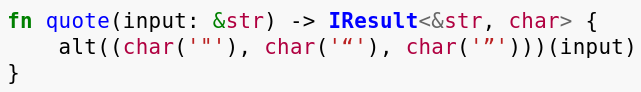
\includegraphics[width=\textwidth]{initial_quote}
	\caption[Screenshot of the initial quote parser supporting all three types of quotes]{Screenshot\footnotemark{} of the initial quote parser supporting all three types of quotes}
	\label{fig:quote_parser}
\end{figure}

\footnotetext{A screenshot had to be taken because we had trouble showing slanted quotes in this document}

\begin{listing}
	\begin{minted}{rust}
#[test]
fn variable_test() {
	assert_eq!(
		program(include_str!("../tests/variable.input")).unwrap().1,
		include!("../tests/variable.ast")
	);
}
	\end{minted}
	\caption{Our very first test}
	\label{lst:first_test}
\end{listing}

\begin{figure}
	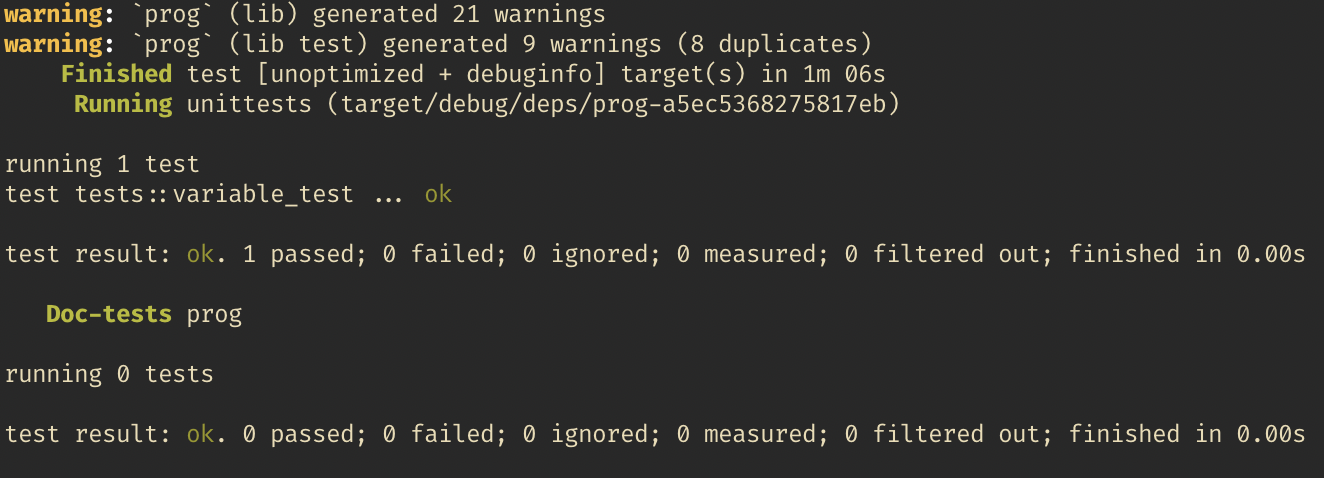
\includegraphics[width=\textwidth]{stage1_test}
	\caption{Screenshot of the first test passing}
	\label{fig:stage1_test}
\end{figure}

\subsection{Stage 2}

In the second stage of development we added more tests and generalised our
testing using metaprogramming\footnote{metaprogramming is when code is written
that generates further code, in our case this was done through rust's macro
system} such that test were not manually written but generated automatically.
This allows us to add tests rapidly and in a reliable way. Now it was possible
to just add tests by adding an entry in the ``tests'' directory and then
referencing it in our code with \mintinline{rust}{ast_test!()}, see listing
\ref{lst:macro_test}. Evidence of the tests passing can be found in
\autoref{fig:stage2_test}. The actual content of the tests can be found in the
final code listing in \autoref{sec:final_project} on page
\pageref{sec:final_project}.

\begin{listing}
	\begin{minted}{rust}
macro_rules! ast_test {
	( $function_name:ident ) => {
		#[test]
		fn $function_name() {
			assert_eq!(
				program(include_str!(concat!(
					"../tests/",
					stringify!($function_name),
					".input"
				)))
				.unwrap()
				.1,
				include!(concat!("../tests/", stringify!($function_name), ".ast"))
			);
		}
	};
}

ast_test!(variable);
ast_test!(variable_quotes);
ast_test!(variable_whitespace);
	\end{minted}
	\caption{The definition of the ast\_test macro and the subsequent use of
	it to define three tests}
	\label{lst:macro_test}
\end{listing}

\begin{figure}
	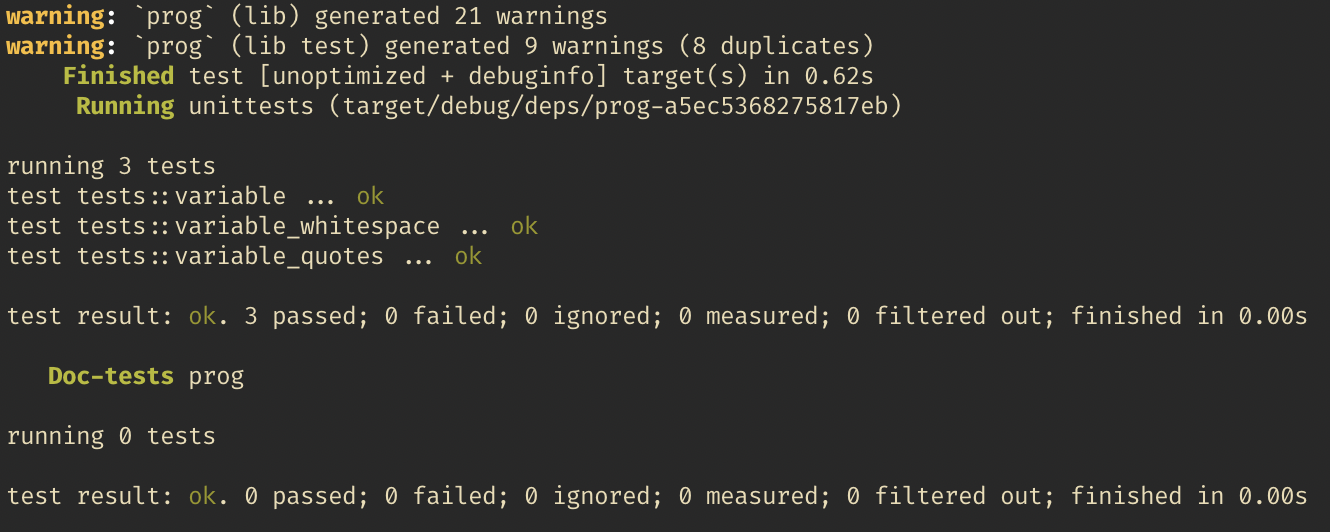
\includegraphics[width=\textwidth]{stage2_test}
	\caption{Screenshot of two new added tests passing}
	\label{fig:stage2_test}
\end{figure}

\subsection{Stage 3}

We then added support for more language constructs to the parser, namely:
function calls, float literals and for loops.

Previously the integer literal variant was called \texttt{NumberLiteral} and so
we renamed it to \texttt{IntegerLiteral} so it wouldn't be confused with
\texttt{FloatLiteral} because a number could be a float or an integer. For the
float implementation we decided to store it as an \texttt{f64}\footnote{This
type is often known as a \texttt{double} in other languages and represents a
64bit floating point number} instead of an \texttt{f32} to have more
flexibility and because the overhead caused by using a larger float wasn't too
much of an issue as this was not a performance critical language.

We also improved our parser for quotes so that what was considered a quote (for
parsing string literals) was stored as a constant which multiple functions
could refer to rather than it being hard-coded (see \autoref{fig:new_quote}).
This approach is more modular and maintainable.

Once again we added tests before implementing the features and
\autoref{fig:stage3_test} shows the tests passing. The tests can be found in
the final project listing.

\begin{figure}
	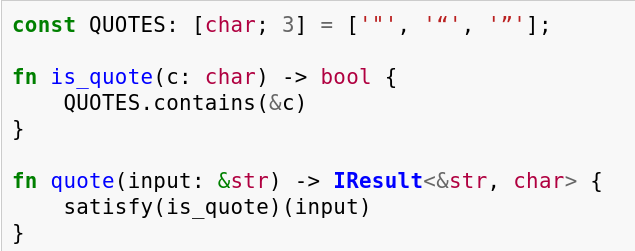
\includegraphics[width=\textwidth]{new_quote}
	\caption{New quote parsing code}
	\label{fig:new_quote}
\end{figure}

\begin{figure}
	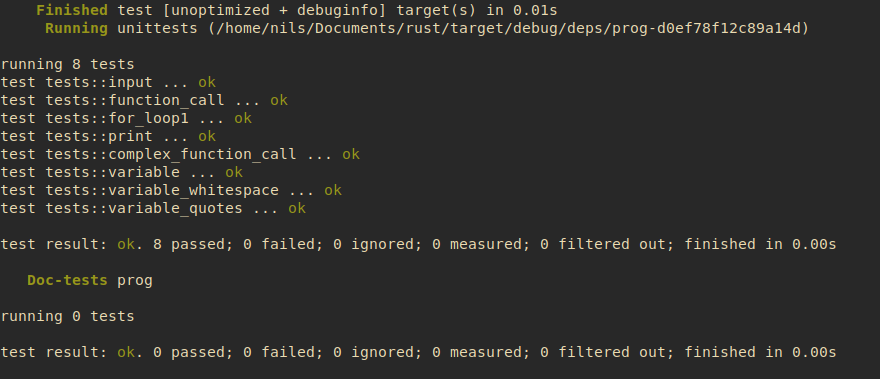
\includegraphics[width=\textwidth]{stage3_test}
	\caption{Tests passing after adding the features}
	\label{fig:stage3_test}
\end{figure}

\subsection{Stage 4}

In stage 4, we added arithmetic and logical operators. It worked for the most
part except that operator precedence didn't work: all operators were treated as
equal and parsed from left to right which caused some unexpected results (see
\autoref{fig:precedence_test_fail}. We decided to follow python's operator
precedence however we weren't sure how to implement it
\cite{python_precedence}.

\begin{figure}
	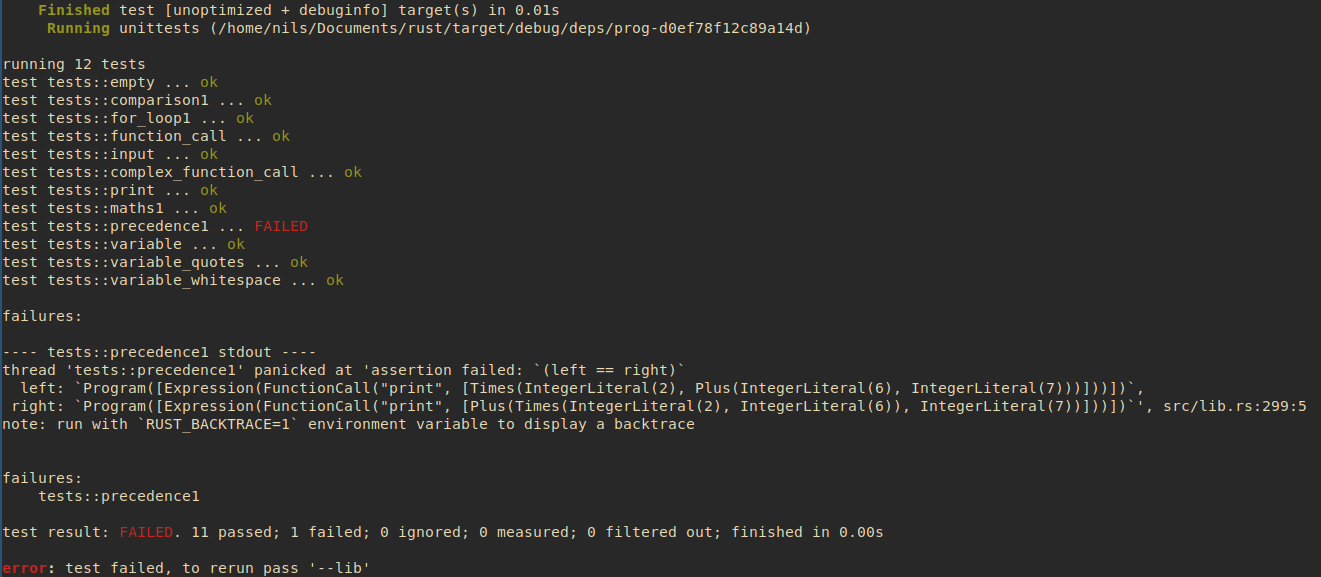
\includegraphics[width=\textwidth]{precedence_test_fail}
	\caption{Screenshot of the precedence1 test failing}
	\label{fig:precedence_test_fail}
\end{figure}

After doing some research and looking at existing examples of precedence
parsing using the \citetitle{nom} library we found out that one possible way to
do it was by parsing in layers of different recursion depth, first parsing the
operators with the least precedence and then parsing operators with a greater
precedence from then on. This lead to having multiple depth of parsing called
depth1, depth2, depth3, depth4, depth5, depth6 and terminal. This method worked
and allowed our tests to pass (see \autoref{fig:precedence_test_pass}) however
it increased the amount of code by a lot and made the codebase harder to
navigate compared to our previous attempt using metaprogramming to generate the
parsing code. It also meant that if we were to add another parsing depth we
would need to rename a lot of function or have functions that didn't follow the
current numeral naming scheme.

\begin{figure}
	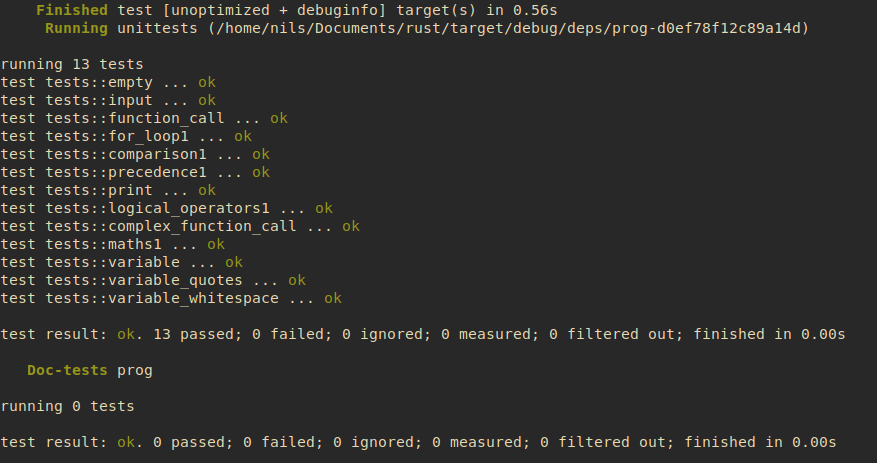
\includegraphics[width=\textwidth]{precedence_test_pass}
	\caption{Screenshot of the precedence1 test passing}
	\label{fig:precedence_test_pass}
\end{figure}

As you can see from \autoref{fig:precedence_test_fail}, failing tests can be
difficult to comprehend because everything is on one line. This is why we
decided to add \citetitle{rust_pretty_assertions} to our dependencies. This is
a library that works similar to rusts \texttt{assert\_eq} macro except it
compares to left and right side when they are not equal making the output more
readable and easier to reason about.

\subsection{Stage 5}

We then went on to implement parsing for the not operator, while loops, if and
switch statements, comments, functions and procedures. In order to implement
comments we had to change our whitespace function so that it would work if
whitespace included comments. An other thing that wasn't defined in the OCR
specification was what was considered to be whitespace. We decided that we
would use whatever was defined as whitespace by \citetitle{nom} which are
spaces, tabs, carriage returns and line feeds. The passing tests can be seen
in \autoref{fig:stage5_test}.

\begin{figure}
	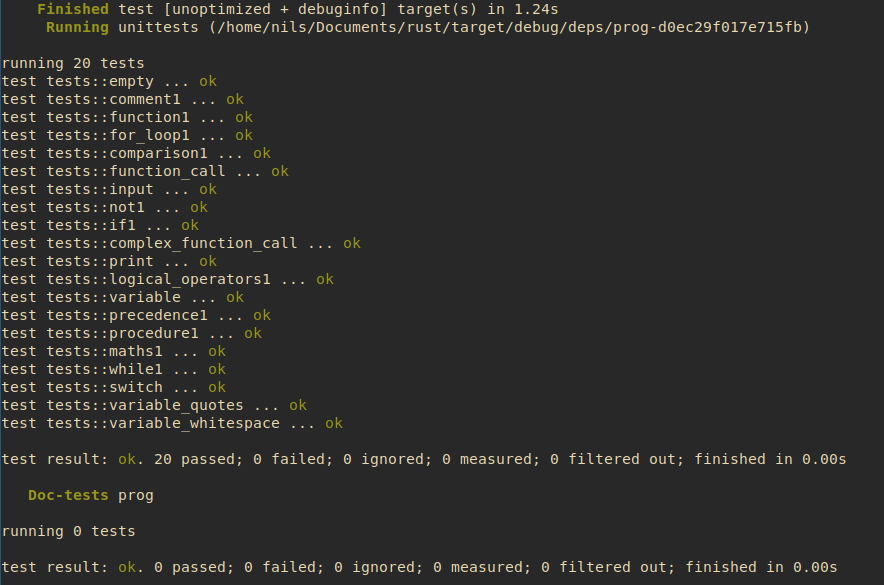
\includegraphics[width=\textwidth]{stage5_test}
	\caption{Screenshot of tests passing for stage 5 of development}
	\label{fig:stage5_test}
\end{figure}

In order to implement \texttt{elseif} and \texttt{switch} statements we made it
such that the results are transformed into a chain of if and else statements.
This allows to simplify our interpreter and improves the performance of our
program at the cost of a slightly more complex parser. Listing
\ref{lst:switch_tranformation} shows how the first two pieces of code are
equivalent to the third whilst using only \texttt{if} and \texttt{else}
statements. A downside to this approach is that as it stands an expression that
takes a long time to compute is given to a switch statement, that expression
will be executed multiple times leading to performance loss and unintended
behaviour if the expression causes side effects.

\begin{listing}
	\begin{minted}{text}
// Using if, elseif and else
if entry == "a" then
	print("You selected A")
elseif entry == "b" then
	print("You selected B")
else
	print("Unrecognised selection")
endif

// Using switch
switch entry:
	case "A":
		print("You selected A")
	case "B":
		print("You selected B")
	default:
		print("Unrecognised selection")
endswitch


// Using just if and else
if entry == "a" then
	print("You selected A")
else
	if entry == "b" then
		print("You selected B")
	else
		print("Unrecognised selection")
	endif
endif
	\end{minted}
	\caption{Three different ways to write the equivalent code}
	\label{lst:switch_tranformation}
\end{listing}

\subsection{Stage 6}

In stage 6, we improved the code quality of our parser in preparation for the
implementation of the interpreter. To make our project more robust we also
added some tests including one from exercises we were given in class. However,
one of them used the \texttt{step} operation in a for loop something which was
first defined in \citetitle{j277}. Because the \texttt{step} feature had not
been implemented yet it resulted in our test failing to compile as can be seen
in \autoref{fig:thinking_logically_failing}.

\begin{figure}
	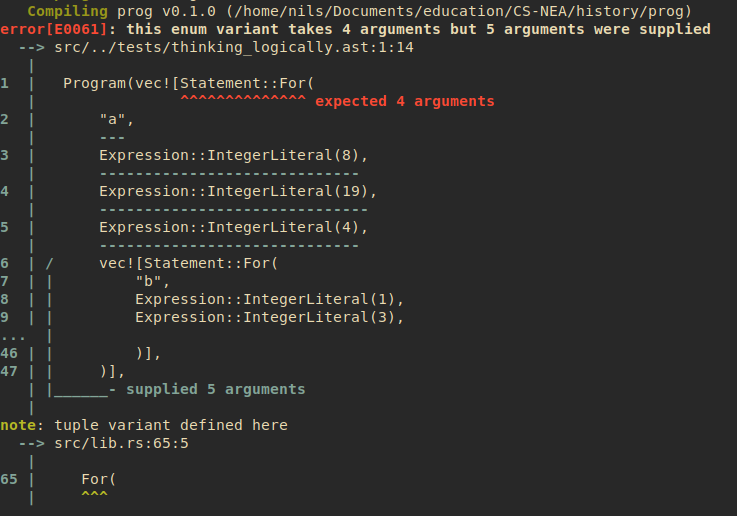
\includegraphics[width=\textwidth]{thinking_logically_failing}
	\caption{Screenshot of tests failing to compile due to the \texttt{step}
	feature not being implemented}
	\label{fig:thinking_logically_failing}
\end{figure}

In order to fix that we implemented the \texttt{step} feature however the test
still wouldn't pass because our implementation for comments didn't support
multiple comments. We also implemented parsing settings simultaneously which
allowed our parser to behave differently based on certain settings such as
whether keywords and variables are case sentitive or not. Unfortunately this
caused a regression which caused the precedence to fail as can be seen in
\autoref{fig:regression}.

\begin{figure}
	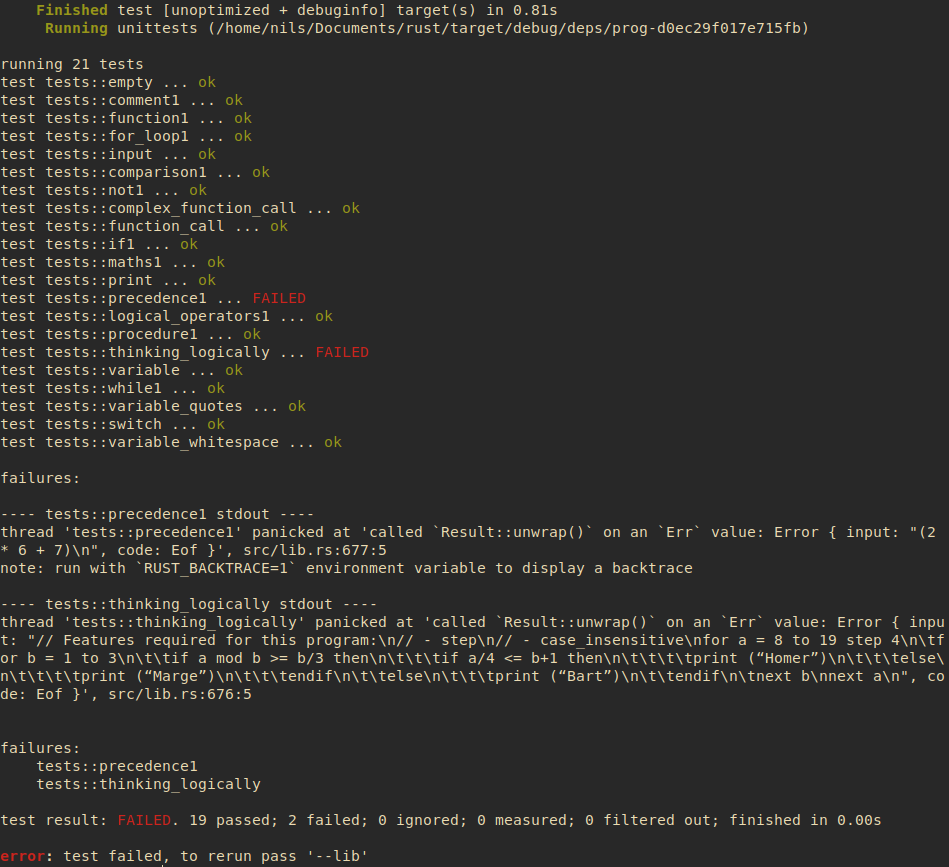
\includegraphics[width=\textwidth]{regression}
	\caption{Screenshot of tests failing due to regression in whitespace
	parsing and multiple comments not being implemented}
	\label{fig:regression}
\end{figure}

Finally, we fixed the regression and implemented the ability to have multiple
comments within one set of whitespace which fixed our tests as can be seen in
\autoref{fig:thinking_logically_passing}.

\begin{figure}
	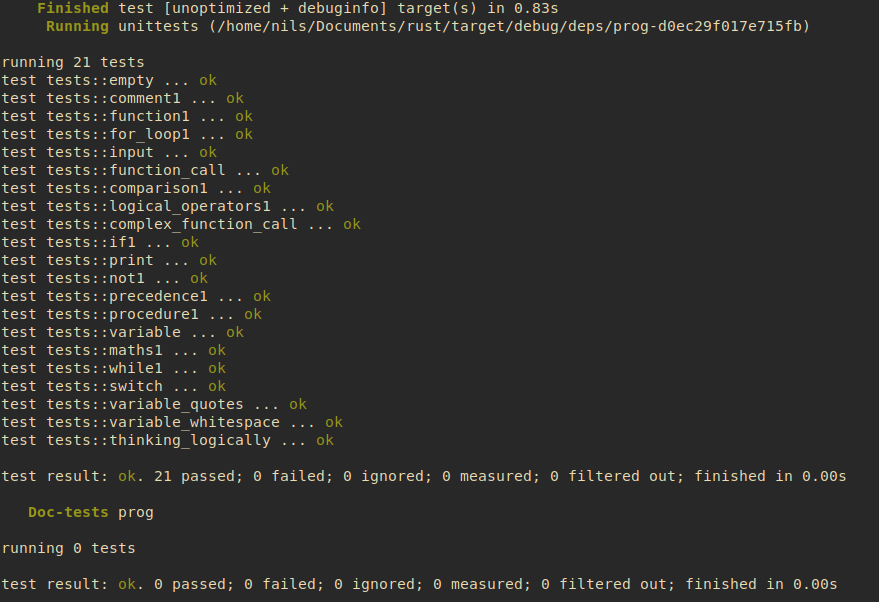
\includegraphics[width=\textwidth]{thinking_logically_passing}
	\caption{Screenshot of tests passing after implementing the \texttt{step}
	feature}
	\label{fig:thinking_logically_passing}
\end{figure}

We also improved the parsing of operators by using a recursive approach instead
of an iterative one avoiding allocations on the heap to store the results. We
also improved code quality by applying the suggestions given by
\citetitle{clippy}\footnote{Rust tool that offers suggestions to improve code
quality}. Another feature of our modular parsing which allows to have different
parsing settings is that it allowed to have looser rules around for loops. In
the OCR Reference language, for loops are terminated using ``next x'' however
in these call specifying the variable is not necessary. With the setting
\texttt{for\_next\_not\_enforced} it is possible to accept programs that don't
have the right matching variable in their \texttt{next} statement.

In order to implement settings we had to turn every single of our parsing
functions into combinators that returned a parser and that accepted settings as
arguments. This meant a major rewrite of our parser because every function had
to be changed. Listing \ref{lst:settings_expression} shows an example of how a
small parser had to be changed, this operation had to be done for the entirety
of our parser. Listing \ref{lst:tag_with_settings} shows an example of a parser
now taking into account settings.

\begin{listing}
	\begin{minted}{diff}
-fn expression(input: &str) -> IResult<&str, Expression> {
-    depth1(input)
+fn expression(
+    parse_settings: &ParseSettings,
+) -> impl FnMut(&str) -> IResult<&str, Expression> + '_ {
+    depth1(parse_settings)
 }
	\end{minted}
	\caption{Adding settings to the expression parser}
	\label{lst:settings_expression}
\end{listing}

\begin{listing}
	\begin{minted}{rust}
fn tag_with_settings<'a>(
    tag_str: &'a str,
    parse_settings: &'a ParseSettings,
) -> impl FnMut(&str) -> IResult<&str, &str> + 'a {
    move |input: &str| {
        if parse_settings.case_sensitive {
            tag(tag_str)(input)
        } else {
            tag_no_case(tag_str)(input)
        }
    }
}
	\end{minted}
	\caption{A combinator returning a parser that takes into account settings}
	\label{lst:tag_with_settings}
\end{listing}

\subsection{Stage 7}

In stage 7, we added a basic interpreter to our language. As part of that we
modularised our code moving parser related code to \texttt{parser.rs} and
interpreter related code to \texttt{interpreter.rs}. As part of this stage we
also added a simple CLI interface so that it was possible to run code from the
command line. This parser could only implement a limited set of statements and
was designed to run the thinking logically test.

\subsection{Stage 8}

For stage 8 we continued adding features to the parser and adding tests. We
added support for \texttt{do} \texttt{until} statements, array declaration and
object-oriented related features (method parsing, class parsing, object
instantiation parsing).

We also improved performance by using binary search to find if a word was a
keyword instead of our previous naive linear search. For binary search to work
we have to make sure the list of keywords is sorted at all time something we
can do with a test which can be seen in listing \ref{lst:sorted_keywords}. You
may notice that the list of keywords almost only includes keywords that end
statements. The reason for this is that when parsing there is only ambiguity
when parsing endings so it is not necessary to have beginning keywords in the
list of keywords.

\autoref{fig:stage8_test} shows the tests passing after adding many tests and
the features discussed in this section.

\begin{figure}
	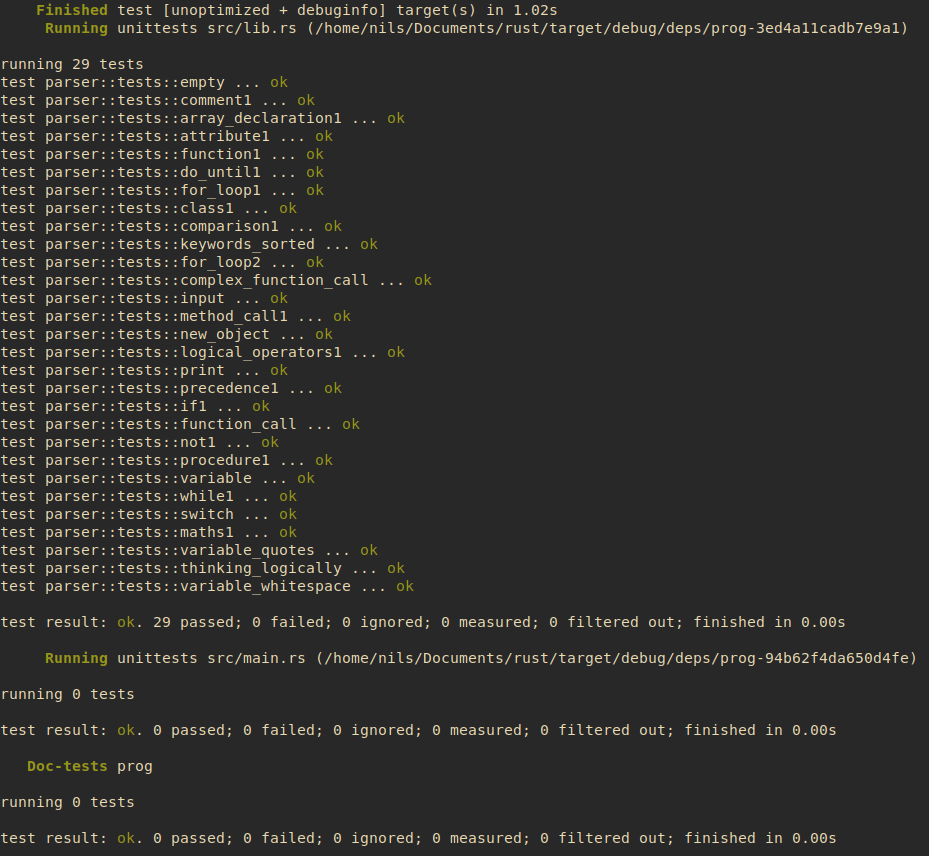
\includegraphics[width=\textwidth]{stage8_test}
	\caption{Screenshot of tests passing after implementing more features in
	the parser}
	\label{fig:stage8_test}
\end{figure}

\begin{listing}
	\begin{minted}{rust}
const KEYWORDS: [&str; 14] = [
    "case",
    "default",
    "else",
    "elseif",
    "endclass",
    "endfunction",
    "endif",
    "endprocedure",
    "endswitch",
    "endwhile",
    "function",
    "next",
    "procedure",
    "until",
];

#[test]
fn keywords_sorted() {
	assert!(KEYWORDS.is_sorted());
}
	\end{minted}
	\caption{Test making sure keywords are sorted for parsing}
	\label{lst:sorted_keywords}
\end{listing}

\subsection{Stage 9}

For stage 9, we made changes that allowed our interpreter to be more than just
a toy to be able to execute a single piece of code. To do that we redid the
value system by having two types of values: DenotedValue and Value.
DenotedValue is the type of values that are stored in the environment, it is
nothing more than an Value inside of a RefCell inside of an Rc type. Value
is the type defining the actual different types our programming language can
take.

In rust the Rc type allows to store reference counted items on the heap and
RefCell allows to have interior mutability: it allows to mutate values without
it being checked by the borrow checker. These types are necessary because in
rust the borrow checker prevents values from being mutated if there are other
references to a value. The RefCell type allows to maintain that guarantee by
doing the checks at runtime. We used the Rc type because it is necessary in
order to not use too much memory: it destroys objects if there are no
references to it.

We also moved all code related to values to a separate file: \texttt{value.rs}.
We also added the macro necessary to be able to add tests rapidly to the parser
(the macro can be seen in listing \ref{lst:output_test}. The way this macro
works is that it executes the code in \texttt{.input} files and then compares
the output produced with files in \texttt{.output} files. If the output
matches, the test passes.

\begin{listing}
	\begin{minted}{rust}
macro_rules! output_test {
    ( $function_name:ident ) => {
        #[test]
        fn $function_name() {
            let mut stdout = Vec::new();
            Program::from_str(
                include_str!(concat!(
                    "../test_data/",
                    stringify!($function_name),
                    ".input"
                )),
                &ParseSettings::default(),
            )
            .unwrap()
            .interpret_with_write(&mut stdout);
            print!("{}", std::str::from_utf8(&stdout).unwrap());
            assert_eq!(
                stdout,
                include_bytes!(concat!(
                    "../test_data/",
                    stringify!($function_name),
                    ".output"
                ))
            );
        }
    };
}
	\end{minted}
	\caption{The macro used for testing the interpreter part of the programming
	language}
	\label{lst:output_test}
\end{listing}

As part of this stage we added many features. We implemented printing such that
values of different types could be printed and such that the output of printing
could be captured. We did this by having our interpreter accept an object that
implements the \texttt{Write} trait. On the command line, the object passed is
an instance of standard output. In tests it is a Vec, such that we can collect
the results for later.

Because we now have tests for the interpreter we will only show screenshots of
a subset of the tests so as to not crowd this report with information that is
not necessary as there are now too many tests to show them all at once.
Nevertheless we will run the full test suite as we develop the programming
language to make sure no bugs are introduced by.
\autoref{fig:stage9_test} shows the tests that were added as part of stage 9
passing.

\begin{figure}
	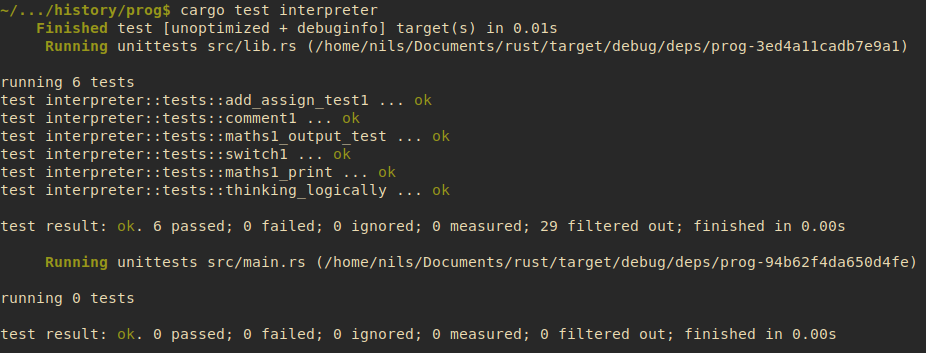
\includegraphics[width=\textwidth]{stage9_test}
	\caption{Screenshot of tests passing at the end of stage 9}
	\label{fig:stage9_test}
\end{figure}

% Stage 10
\subsection{Stage \subsecnum}

For stage \subsecnum, we started the playground, a web application that allows
to use the programming language from one's browser.

This first version was very basic, it had a \texttt{textarea} for the user's
code and would just output to the web page through a \texttt{output} tag to
achieve a monospaced formatting. A problem this version had is that it couldn't
print in real time. The web page was only updated once the program had finished
executing due to the web's asynchronous architecture: when the user's program
was running, its execution was blocking the DOM from being refreshed.

\autoref{fig:webappv1} shows running a small test program on the web
application.

\begin{figure}
	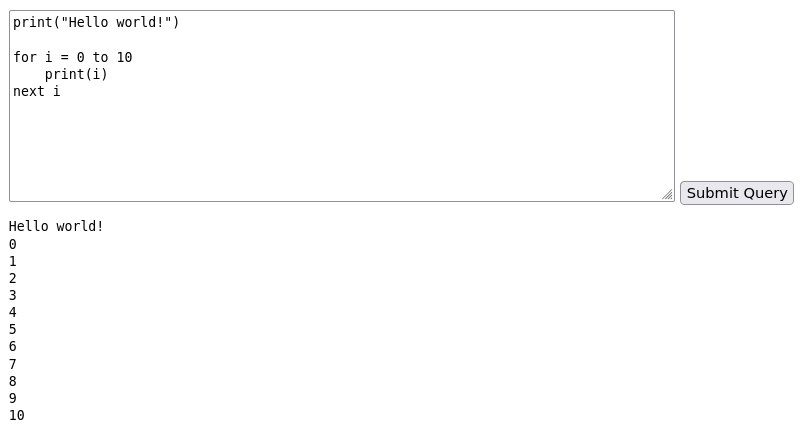
\includegraphics[width=\textwidth]{webappv1}
	\caption{Screenshot of the first version of the playground}
	\label{fig:webappv1}
\end{figure}

% Stage 11
\subsection{Stage \subsecnum}

For stage \subsecnum, we tried desperately to be able to print continuously in
real time, such as within an infinitely running loop. We went through different
iterations and methods before we achieved something that worked in a robust
way.

We thought that using the xterm.js package would allow use to print in real
time, it didn't work. In hindsight there was no reason why using it would solve
our solution. We also tried many workarounds that we thought would introduce a
pause in the page leaving enough time for the DOM to refresh, these include
calling \mintinline{javascript}{window.requestAnimationFrame()}, calling
\mintinline{javascript}{setTimeout()}, changing the visibility of the output
to \texttt{none} and then back to \texttt{block}, or requesting the
\texttt{offsetHeight} attribute of the output after each print. None of them
worked.

In the end what we did is we made the program run in a web worker, a separate
virtual page independent from the main web page and which communicates with the
main web page by passing messages to each other. After this change it was now
possible to print to the screen continuously in real time.

This can be tested by running a very simple infinite loop in the playground
such as the one in listing \ref{lst:infinite_loop}.

\begin{listing}
	\begin{minted}{text}
a = 1
while True
    print(a)
    a = a + 1
endwhile
	\end{minted}
	\caption{Infinite loop program to test continuous real-time printing in the
	playground}
	\label{lst:infinite_loop}
\end{listing}

Whilst working on this feature, we reached another bug, output from the web
worker would be corrupted. We are not sure why that is the case however we were
able to solve it by calling \texttt{slice} on the output before sending it to
the main thread. We believe that the reason \texttt{slice} fixes the bug is
that it makes a new copy of the data, however we do not understand why it is
necessary as the data should not be mutated after it is sent as a message. This
workaround probably has a negative impact on performance as it leads to data
being copied and allocated.

% Stage 12
\subsection{Stage \subsecnum}

For stage \subsecnum, we added more features to the playground: the ability to
stop a program using CTRL-C like in a normal terminal, a button to print the
AST of a program and lastly we changed the editor from a \texttt{textarea} to
using the \citetitle{monaco}, the same one that is used in \citetitle{vscode}.
\autoref{fig:monaco} shows a screenshot of the playground after these changes
were implemented.

\begin{figure}
	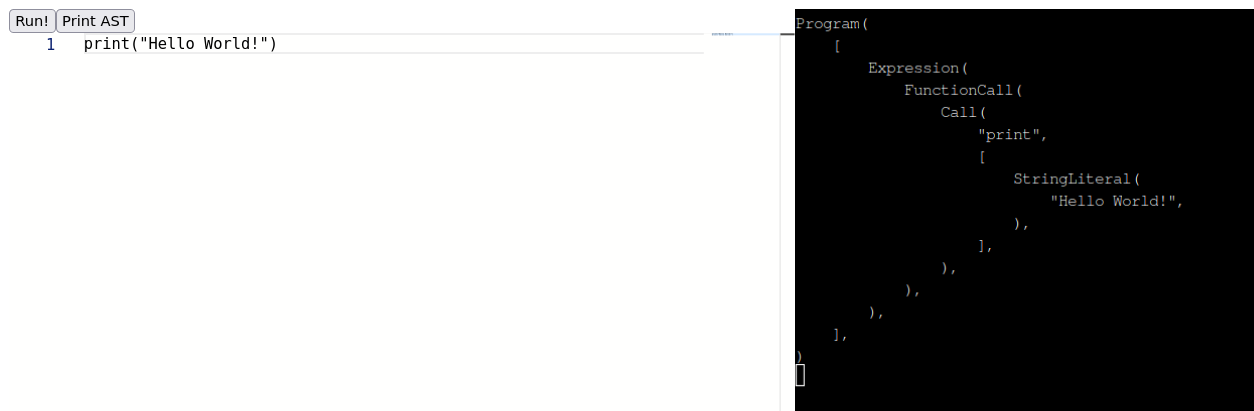
\includegraphics[width=\textwidth]{monaco}
	\caption{Screenshot showing the updated playground with monaco editor on
	the left and the AST on the right}
	\label{fig:monaco}
\end{figure}

% Stage 13
\subsection{Stage \subsecnum}

For stage \subsecnum, we made improvements to the interpreter: we added support
for boolean and real literals, logical operators, and while loops in the
interpreter. We also fixed a bug in the parser that made it so that numbers
that started with a minus sign were parsed as identifiers instead of integers
or real numbers. We added tests to make sure this was not going to regress and
others for the features listed.

\begin{figure}
	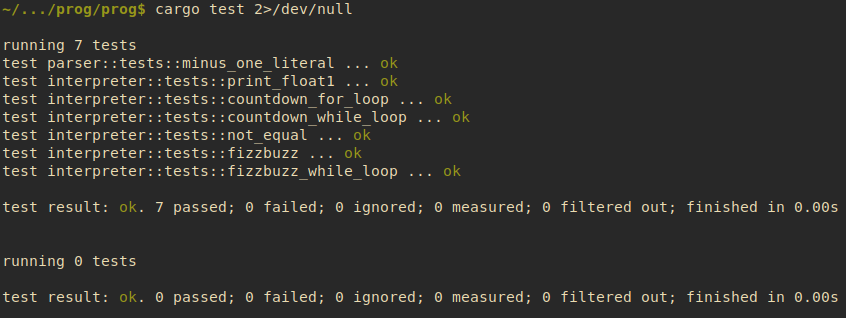
\includegraphics[width=\textwidth]{stage13_test}
	\caption{Screenshot of tests passing after the changes of stage 13 have
	been carried out}
	\label{fig:stage13_test}
\end{figure}

\autoref{fig:stage13_test} shows the tests that were added passing after the
changes have been implemented.

% Stage 14
\subsection{Stage \subsecnum}

For stage \subsecnum, we added support for arrays in the interpreter. We also
improved our implementation of for loops by mutating a reference to the counter
variable rather than inserting the counter variable into the stack on each
iteration. This has the downside that if a program changes the counter
variable, it will not be reset to the value it should have, something that may
be beneficial or not depending on the context.

We implemented multi-dimensional arrays as arrays of arrays which gives us a
lot of flexibility. Additionally arrays can contain values of any type and do
not have to contain only a single type. This follows our philosophy of
accepting as much code as possible, something we have to do because of how
loosely the language is defined by OCR.

As part of this stage we also implemented string concatenation, something that
is necessary for printing as well as the \texttt{do}-\texttt{until} loop. The
tests added as part of this stage can be seen to pass in
\autoref{fig:stage14_test}. We didn't add tests for \texttt{do}-\texttt{until}
loops because we haven't implemented \texttt{input} yet. When we will implement
the \texttt{input} function, we will then add the appropriate tests.

\begin{figure}
	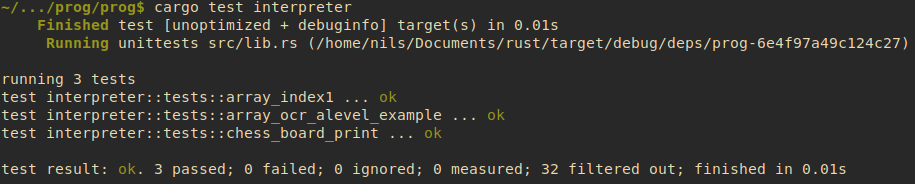
\includegraphics[width=\textwidth]{stage14_test}
	\caption{Screenshot of tests for stage 14 passing}
	\label{fig:stage14_test}
\end{figure}

% Stage 15
\subsection{Stage \subsecnum}

For stage \subsecnum, we did one of the biggest changes to our language, we
implemented classes and objects. In order to implement them we changed some of
the core functions of the interpreter, such as the \texttt{eval} function which
evaluates an expression within a given context to return a raw Value, not a
reference like it used to and we added a function \texttt{get\_ref} which
returns a reference instead of a value. As part of these changes we had to
change the AST, which is quite unfortunate because it meant rewriting almost
all of our \texttt{.ast} files making this stage even more complex.

Some of the changes to the AST made it more consistent by for example having
attributes be references which had as parent the expression before the full
stop, and a subroutine call being a call on a reference. This was quite complex
as it meant making more parts of our parser recursive which as we explored
before is not easy to implement.

\autoref{fig:stage15_test} shows the tests testing the features implemented in
this stage passing.

\begin{figure}
	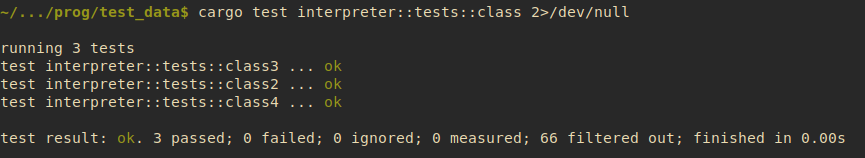
\includegraphics[width=\textwidth]{stage15_test}
	\caption{Screenshot of tests for classes and objects passing}
	\label{fig:stage15_test}
\end{figure}

\subsection{Stage \subsecnum}

For stage \subsecnum, we added the possibility to use single quotes as quotes
for string literals, similarly to languages such as \citetitle{javascript} and
\citetitle{python} where single quotes and double quotes are entirely
equivalent in semantics. This feature was put behind a feature flag because it
is a deviation of the language defined by OCR.

We also added support for basic functions, by executing their bodies when a
function call is executed and making \texttt{execute\_statements} return a
Value, although for the moment we have left it as returning Undefined.

Last but not least, we implemented the \texttt{input} function for the CLI
interface. We were not able to implement it for the playground because of the
asynchronous nature of \citetitle{javascript} APIs. In order to receive a
message inside of a worker, we need to do so asynchronously something that is
not possible from our synchronous code.

\subsection{Stage \subsecnum}

For stage \subsecnum, we added support to string operations. We decided to implement it
before other built-in features such as file operations because making it work
would be similar to making files work. Another advantage of string operations
is that they were fully lowercase which meant it was easier for us to implement
because of the way case sensitivity is handled: when the programming language
is set to case insensitive mode, it puts everything to lowercase which makes it
difficult to compare in the interpreter section without taking the risk to have
collisions between names. Do note however that in the specification
``substring'' is sometimes written \texttt{substring} and other times
\texttt{subString} so there is really no way of knowing which is correct.

Considering how trivial it was to implement the string operations defined in
\citetitle{h446} (\texttt{substring()} and \texttt{length}) we decided to also
implement the string operations described in \citetitle{j277} (\texttt{left},
\texttt{right}, \texttt{upper}, and \texttt{lower}) along with the tests
necessary. \autoref{fig:string_tests} shows the tests passing.

\begin{figure}
	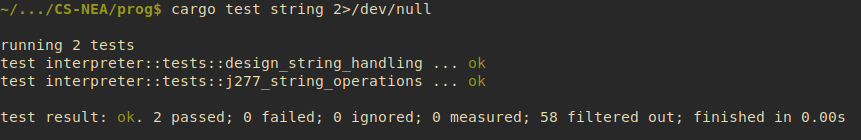
\includegraphics[width=\textwidth]{string_tests}
	\caption{Screenshot tests that make use of string handling passing}
	\label{fig:string_tests}
\end{figure}

\subsection{Stage \subsecnum}

For stage \subsecnum, we implemented the remaining built-in functions for both
\citetitle{j277} and \citetitle{h446}:

\begin{itemize}
	\item The casting functions: \texttt{str}, \texttt{int}, \texttt{float},
		\texttt{real}, \texttt{bool}
	\item ASCII conversion: \texttt{ASC}, \texttt{CHR}
	\item \texttt{random}
\end{itemize}

For a reason we are not aware of, \citetitle{j277} defines both a real and
float casting functions, we will just treat them as redundant functions and
make them do the same thing. As far as we are concerned there is no difference
between a float and a real type.

The ASCII conversion functions also cause an issue in that they do not use only
capital letters which can case an issue when the case insensitive feature is
enabled. The solution we found which wouldn't require rewriting the
\texttt{.ast} files for our existing tests is to transform the functions into
their wanted case during parsing if case insensitive mode is enabled, using a
function \texttt{convert\_case} as can be seen in listing
\ref{lst:convert_case}.

\begin{listing}
	\begin{minted}{rust}
fn convert_case(identifier: &str) -> String {
    let identifier = identifier.to_lowercase();
    match identifier.as_str() {
        "asc" => "ASC".to_string(),
        "chr" => "CHR".to_string(),
        "openread" => "openRead".to_string(),
        "openwrite" => "openWrite".to_string(),
        "readline" => "readLine".to_string(),
        "writeline" => "writeLine".to_string(),
        "endoffile" => "endOfFile".to_string(),
        "newfile" => "newFile".to_string(),
        _ => identifier,
    }
}
	\end{minted}
	\caption[Implementation of the convert\_case function]{Implementation of
	the convert\_case function}
	\label{lst:convert_case}
\end{listing}

\begin{figure}
	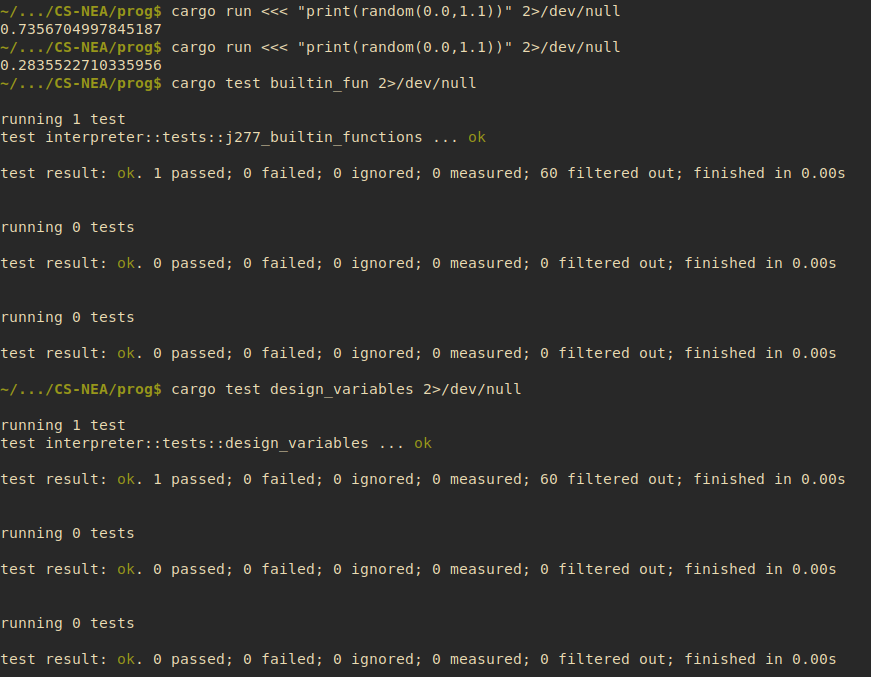
\includegraphics[width=\textwidth]{builtin_functions}
	\caption{Screenshot of tests using builtin functions working}
	\label{fig:builtin_functions}
\end{figure}

\autoref{fig:builtin_functions} shows the built-in functions working.

\subsection{Stage \subsecnum}

For stage \subsecnum, we deployed the web application to GitHub pages using GitHub
actions so that it would deploy automatically when a change is made and so that
the web-app is available to everyone from the internet.

In order to do so, we had to improve our webpack configuration so that it would
copy static files to the \texttt{dist} directory from where we will deploy to
GitHub pages and setup a GitHub workflow so that deployment would happen at
every change. Additionally we separated the CLI interface into a separate crate
so that building the web application would not include dependencies used by the
CLI.

With all of that done, the language is now available from the web! At the
following address: \url{https://prog.tools.nilsand.re/}.

\subsection{Stage \subsecnum}

For stage \subsecnum, we added support for file operations: \texttt{newFile},
\texttt{openRead}, \texttt{readLine}, \texttt{endOfFile}, \texttt{openWrite},
\texttt{writeLine}, \texttt{close}. We will not add support for the
\texttt{open} function defined in \citetitle{j277} because it corresponds to no
known behaviour in other programming languages. The \texttt{open} function
seems to be a read-write open which at the same time appends and starts from
the beginning, something that doesn't make much sense, as such we prefer to
leave it unimplemented, and keep using the functions from the A level
specification.

\autoref{fig:file_test_fail} shows the tests failing before the file operations
are implemented.

\begin{figure}
	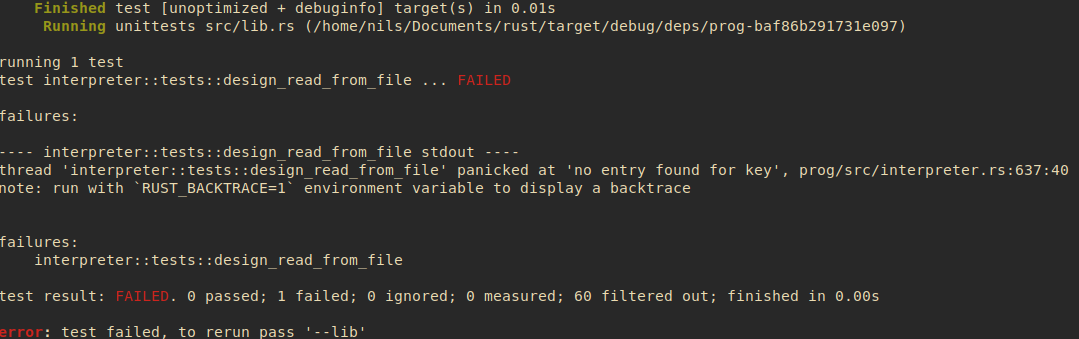
\includegraphics[width=\textwidth]{file_test_fail}
	\caption{Screenshot of test for file operations failing before file
	operations are implemented.}
	\label{fig:file_test_fail}
\end{figure}

Our test has to refer to another file located in the testing directory however
when tests are executed in rust, they are executed from a different working
directory. The recommended method to locate files is to use the
\texttt{CARGO\_MANIFEST\_DIR} environment variable however our language does
not support environment variables. There are multiple methods to fix this
limitation: implement some method to recover environment variables, set the
location using the testing framework or hard-code the location of the file.

We decided to go with the first method by adding the \texttt{system} function
to the language. This function works similarly to how it does in python, PHP or
C: it executes the command given using the default shell (often bash on Linux
and cmd.exe on Windows) and then returns the output of the command. We have
decided to use this method because being able to execute system commands is
necessary for a language to be usable and so we believe that this feature
should be implemented anyway. This will be the first extension to the language
we make. The function \texttt{system} is not defined in any of the documents
produced by OCR.

Because the system function is platform specific we had to implement it in
three different ways depending on the platforms: unix (Linux and MacOS),
windows and Web Assembly using conditional compilation as shown in listing
\ref{lst:system}.

Whilst testing for the file feature we stumbled upon a parsing bug. If an
identifier started with ``new'' our parser would interpret that as an object
instantiation instead of an identifier as can be seen in
\autoref{fig:new_parsing_bug}. We went about fixing it by first adding a test
to make sure the behaviour will stay correct and then fixing the bug.
\autoref{fig:new_bug_fail} shows the test failing before it was fixed and
\autoref{fig:new_bug_success} shows the test succeeding after fixing the
parser.

\begin{figure}
	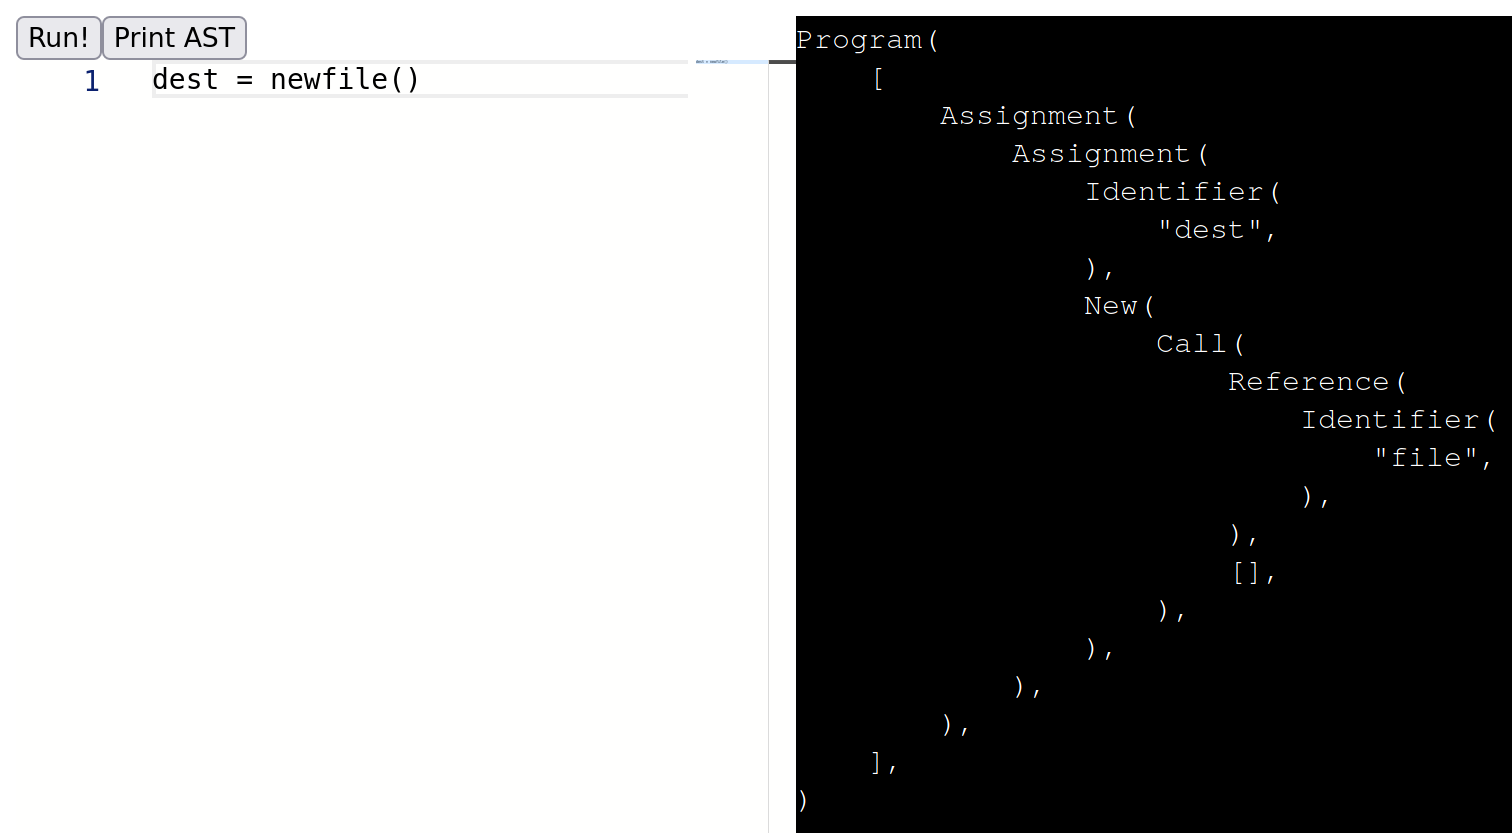
\includegraphics[width=\textwidth]{new_parsing_bug}
	\caption{Screenshot showing an erroneous AST being generated}
	\label{fig:new_parsing_bug}
\end{figure}

\begin{figure}
	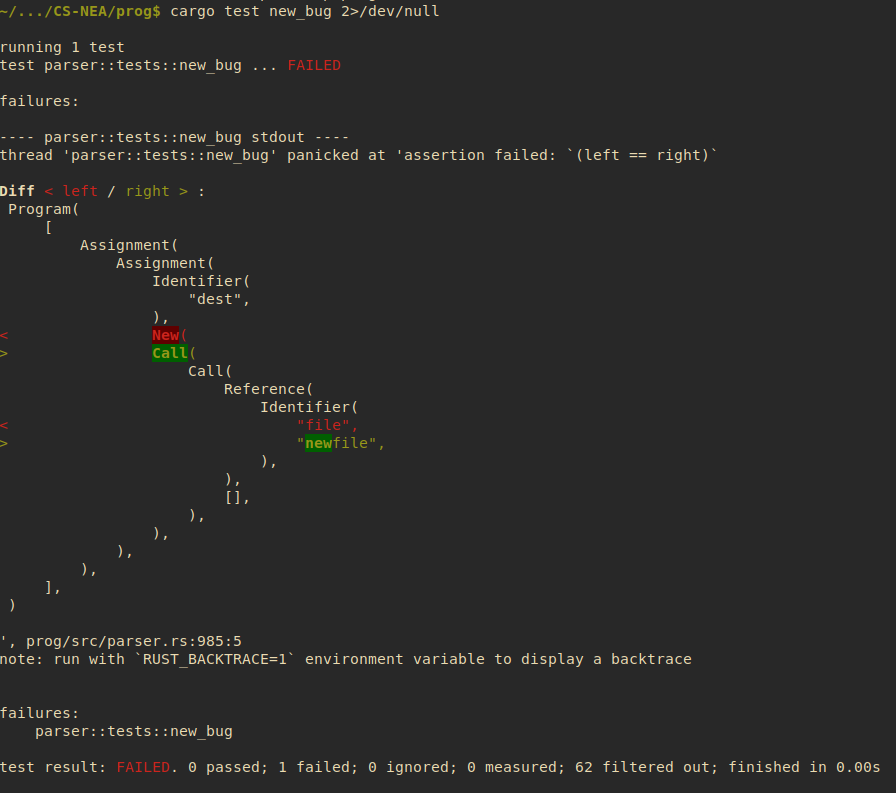
\includegraphics[width=\textwidth]{new_bug_fail}
	\caption{Screenshot of test failing because of erroneous parser}
	\label{fig:new_bug_fail}
\end{figure}

\begin{figure}
	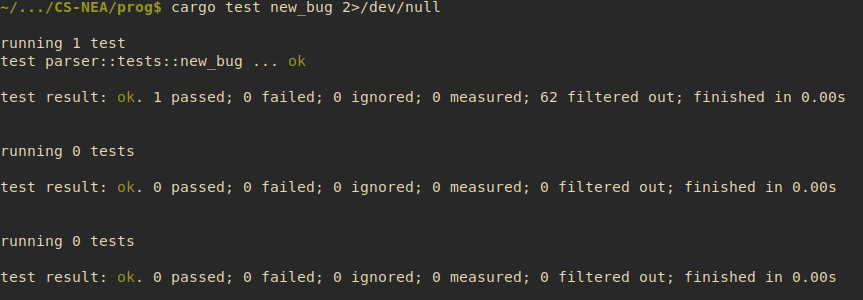
\includegraphics[width=\textwidth]{new_bug_success}
	\caption{Screenshot of succeeding test after fixing parser}
	\label{fig:new_bug_success}
\end{figure}

\begin{listing}
	\begin{minted}{rust}
#[cfg(unix)]
fn system(command: String) -> io::Result<String> {
    use lazy_static::lazy_static;
    use std::process::Command;
    use std::{env, ffi::OsString};

    lazy_static! {
        static ref SHELL: OsString = env::var_os("SHELL").unwrap();
    };

    Command::new(&*SHELL)
        .arg("-c")
        .arg(command)
        .output()
        .map(|output| String::from_utf8(output.stdout).unwrap())
}

#[cfg(windows)]
fn system(command: String) -> io::Result<String> {
    Command::new("cmd")
        .arg("/C")
        .arg(command)
        .output()
        .map(|output| String::from_utf8(output.stdout).unwrap())
}

#[cfg(all(
    target_arch = "wasm32",
    target_vendor = "unknown",
    target_os = "unknown"
))]
fn system(_: String) -> io::Result<String> {
    panic!("system unimplemented for web")
}
	\end{minted}
	\caption{Implementation of the system function}
	\label{lst:system}
\end{listing}

Once everything was implemented, the tests testing the file features succeeded
as can be seen in \autoref{fig:file_success}.

\begin{figure}
	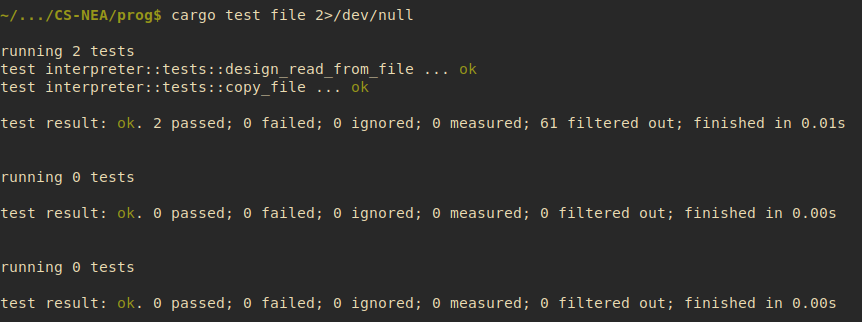
\includegraphics[width=\textwidth]{file_success}
	\caption{Screenshot showing the file related tests succeeding}
	\label{fig:file_success}
\end{figure}

\subsection{Stage \subsecnum}

For stage \subsecnum, we are improving the error messages on the web application.
Currently when an error is reached the user is never informed, all that happens
is that an error message is printed into the developer console of the browser.

In order to fix this issue, we will setup a hook in our code such that when a
panic is reached it will print to the output terminal in a red colour as can be
seen in listing \ref{lst:ansi_printing}. The output can be seen in
\autoref{fig:red_error}.

\begin{listing}
	\begin{minted}{rust}
#[wasm_bindgen]
pub fn init() {
    std::panic::set_hook(Box::new(|info| {
        writeln!(WorkerOutput, "\x1b[31m{}\x1b[39m", info.to_string()).unwrap();
        close();
    }));
}
	\end{minted}
	\caption{Panic hooks which prints panic messages in red to the output}
	\label{lst:ansi_printing}
\end{listing}

\begin{figure}
	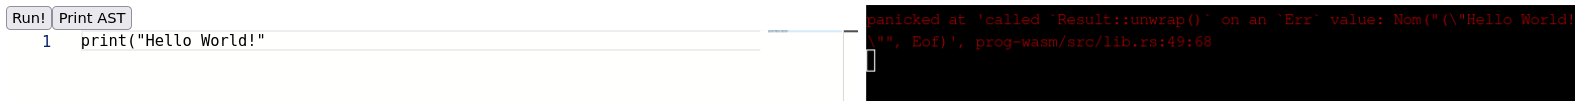
\includegraphics[width=\textwidth]{red_error}
	\caption{Screenshot of error message when there is a syntax error}
	\label{fig:red_error}
\end{figure}

We also removed the scrollbars which were present in previous versions of the
web app by making the size of containers include their padding (scrollbars
visible in \autoref{fig:annoying_scrollbars}). In addition we improved the
code quality to remove the use of absolute values and instead replaced them by
a use of flexbox. This made our web app usable regardless of the screen size it
was used on.

\begin{figure}
	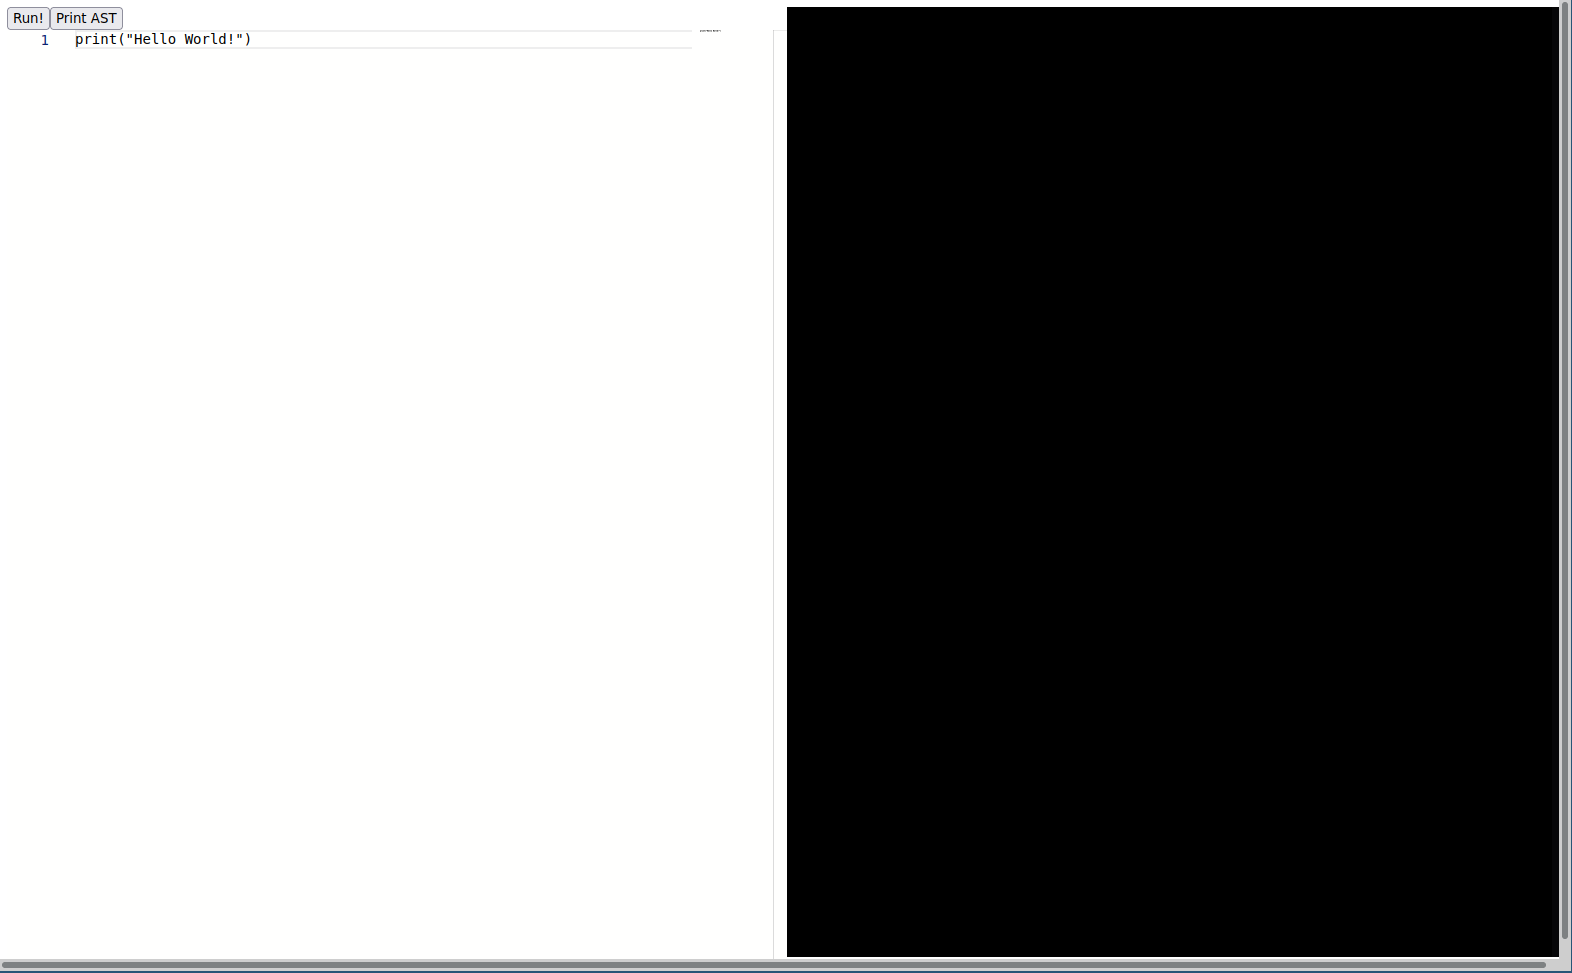
\includegraphics[width=\textwidth]{annoying_scrollbars}
	\caption{Screenshot of the web application before scrollbars were removed}
	\label{fig:annoying_scrollbars}
\end{figure}

% n + 5
\subsection{Stage \subsecnum}

For stage \subsecnum, we will be adding the ability to return values in
sub-blocks of a function. The way we had implemented statements so far meant
that returning values was not something that was possible.

But in order to do that, first we will add tests. We added the \texttt{return1}
and \texttt{return2} tests. The \texttt{return1} test already passed however
the \texttt{return2} didn't pass because its use of return was within a sub
statement. \autoref{fig:return_before} shows the test running before return of
sub-statements was implemented.

\begin{figure}
	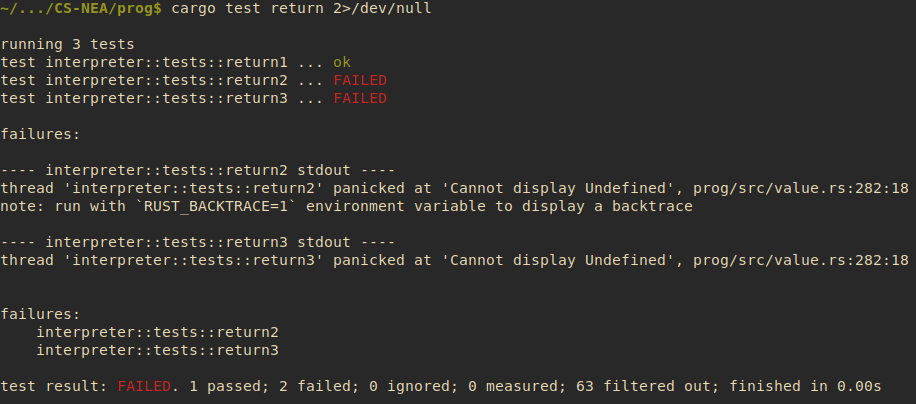
\includegraphics[width=\textwidth]{return_before}
	\caption{Tests for returning values before the feature is complete}
	\label{fig:return_before}
\end{figure}

We were able to implement this feature by using a macro. Using a macro
minimised the amount of code change and made our code more maintainable, both
things which decrease the possibility of a bug occurring. This is a great
example of the use of meta programming and how it can simplify development and
make it elegant and efficient. The macro can be seen in listing
\ref{lst:return_macro}.

\begin{listing}
	\begin{minted}{rust}
// executes the statements returning a value if a value is to be returned
// Otherwise continue
macro_rules! execute_statements {
    ($statements:expr, $context:expr) => {
        match execute_statements($statements, $context) {
            Value::Undefined => (),
            val => return val,
        }
    };
}
	\end{minted}
	\caption{The macro which allows to return values in sub blocks of a
	function}
	\label{lst:return_macro}
\end{listing}

After the changes were made the tests passed as can be seen in
\autoref{fig:return_after}.

\begin{figure}
	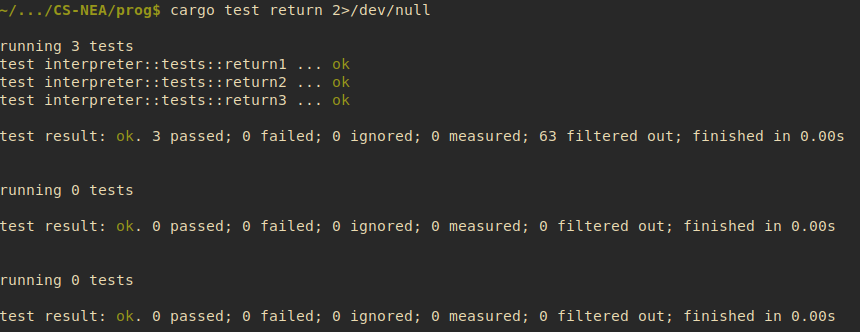
\includegraphics[width=\textwidth]{return_after}
	\caption{Tests for returning values after the feature is complete}
	\label{fig:return_after}
\end{figure}

\subsection{Stage \subsecnum}

For stage \subsecnum, we added an option to display the time it took for a
program to run in the web application. This is useful because it can allow to
take benchmarks and see how efficient and performant the language is, but it
can also indicate when a program has finished executing when said program does
not print anything to the console.

\begin{figure}
	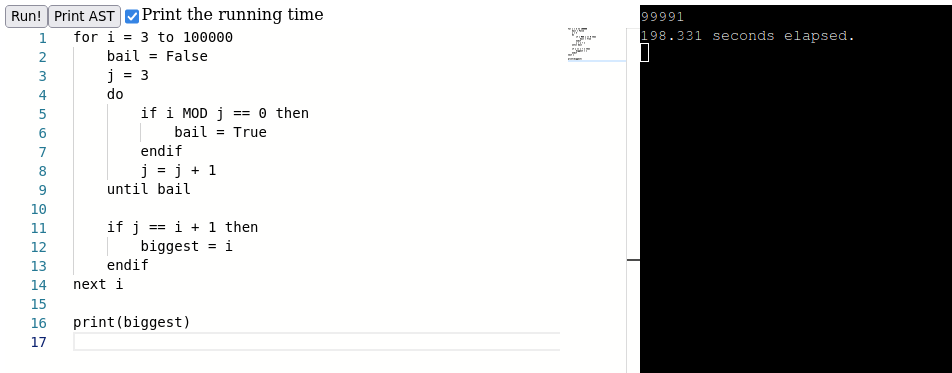
\includegraphics[width=\textwidth]{wasm_prime_bench}
	\caption{Running a benchmark that finds the largest prime smaller than
	100'000 within the playground}
	\label{fig:wasm_prime_bench}
\end{figure}

\autoref{fig:wasm_prime_bench} shows the output once the feature has been added
to the playground.

\subsection{Stage \subsecnum}
\label{sec:better_errors}

For stage \subsecnum, we improved the error messages for missing identifiers.
As it stands when a function or variable is not found the error message gives
little to know useful information as can be seen in \autoref{fig:bad_errors}.

\begin{figure}
	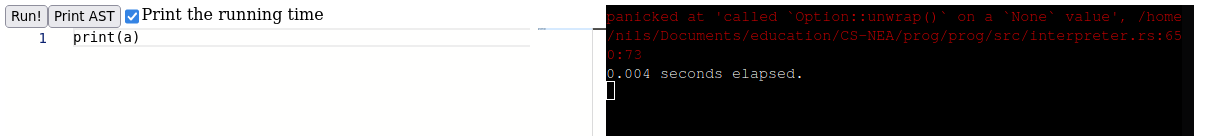
\includegraphics[width=\textwidth]{before_novar}
	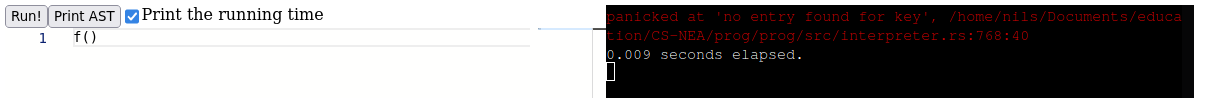
\includegraphics[width=\textwidth]{before_nofunc}
	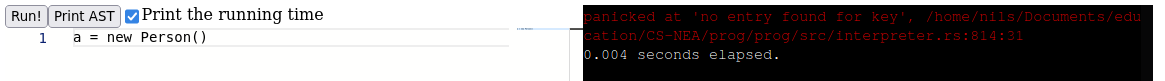
\includegraphics[width=\textwidth]{before_noclass}
	\caption{Screenshot of errors displayed when a function or variable does
	not exist}
	\label{fig:bad_errors}
\end{figure}

\autoref{fig:better_errors} shows error messages after improvements to them.
Although they are not as good as can be seen in mature programming languages,
these error messages are already much better in helping someone attemping to
debug their code.

\begin{figure}
	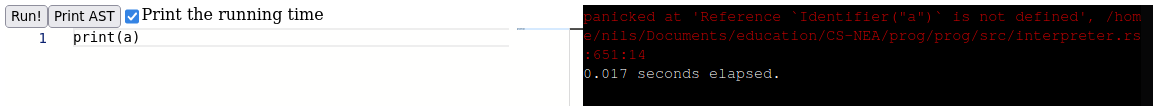
\includegraphics[width=\textwidth]{after_novar}
	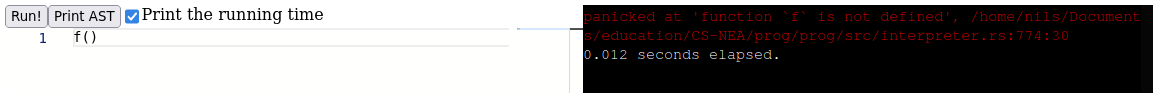
\includegraphics[width=\textwidth]{after_nofunc}
	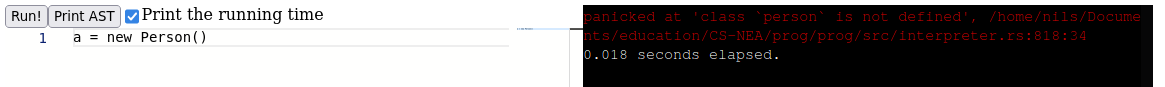
\includegraphics[width=\textwidth]{after_noclass}
	\caption{Screenshot of error messages after improving them}
	\label{fig:better_errors}
\end{figure}

\subsection{Stage \subsecnum}

For stage \subsecnum, we will expose the options to customise the behaviour of
the programming language to users of the playground. For the moment these are
case sensitivity, enforce correct variable after the \texttt{next} keyword of a
for loop, and whether to accept single quotes as valid quotes for strings.
\autoref{fig:playground_options} shows these settings in action.

\begin{figure}
	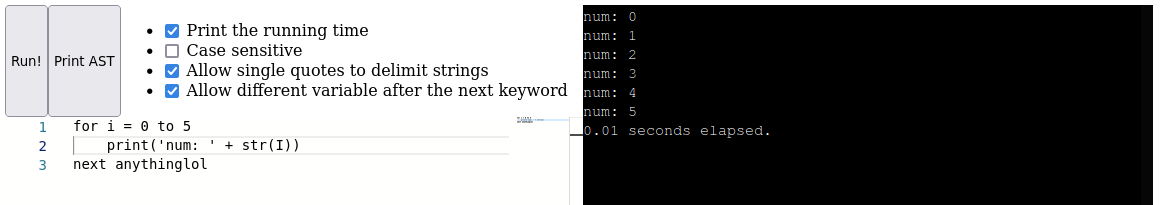
\includegraphics[width=\textwidth]{playground_options}
	\caption{Screenshot of playground with new options}
	\label{fig:playground_options}
\end{figure}

\subsection{Stage \subsecnum}

For stage \subsecnum, we implemented access modifiers for attributes and
methods in the interpreter. Until now, access modifiers were simply ignored for
simplicity. In order to implement access modifiers, we modified the store of
classes in the context to include whether the field was a private field. Whilst
we were at it, we also removed the list of all the fields which is redundant
and used more memory than necessary. We also switched to using a
\texttt{HashMap} to store the fields making field access a lot more efficient
and no longer requiring linear search. For methods, we added an argument to the
\texttt{apply\_method} function which indicate whether this is a call to self
(the current object) or a different object. If it is a call to a different
object, it will fail if the method called is marked as private.

But first, we had to make the test from listing \ref{lst:access_level} be ran
automatically in addition to additional tests. Unlike other tests where we
check whether the program successfully executed and whether the output is
correct, we had to check that the program failed to execute. We were able to do
this using the \mintinline{rust}{#[should_panic]} provided by rust as can be
seen in listing \ref{lst:access_level_test}. \autoref{lst:before_access_level}
shows the test failing before access modifiers are implemented and
\autoref{lst:after_access_level} shows the test succeeding after the
implementation.

\begin{listing}
	\begin{minted}{rust}
#[test]
#[should_panic]
fn access_level() {
    let program = Program::from_str(
        include_str!("../test_data/access_level.input"),
        &ParseSettings::default(),
    )
    .unwrap();
    program.interpret();
}
                                                                 
#[test]
#[should_panic]
fn access_level_methods() {
    let program = Program::from_str(
        include_str!("../test_data/access_level_methods.input"),
        &ParseSettings::reject_single_quote(),
    )
    .unwrap();
    program.interpret();
}
	\end{minted}
	\caption{Code to test access modifiers automatically}
	\label{lst:access_level_test}
\end{listing}

\begin{figure}
	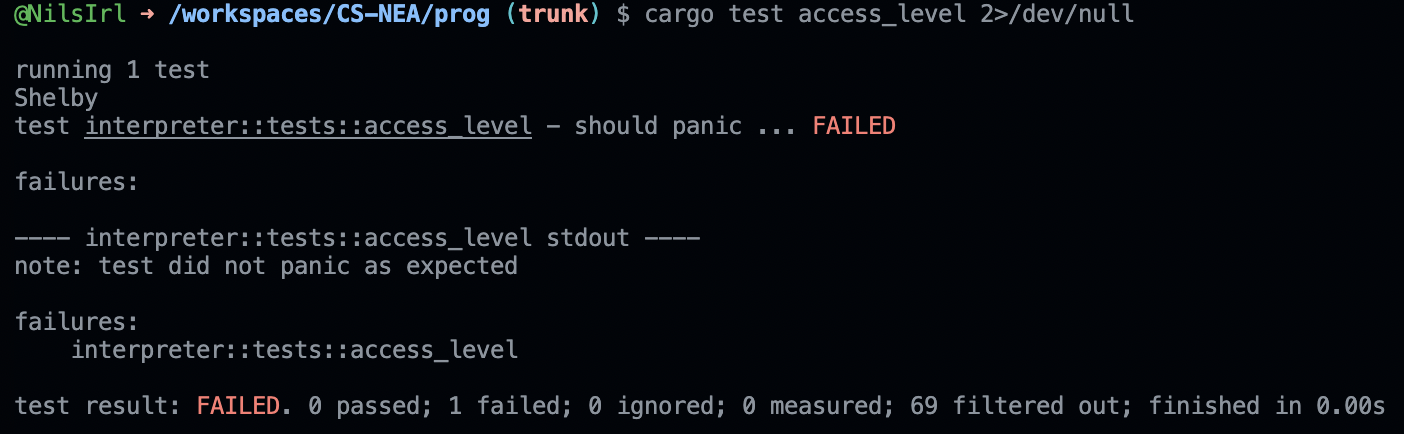
\includegraphics[width=\textwidth]{before_access_level}
	\caption{Screenshot showing the access modifier test failing before access
	modifiers are properly implemented.}
	\label{lst:before_access_level}
\end{figure}

\begin{figure}
	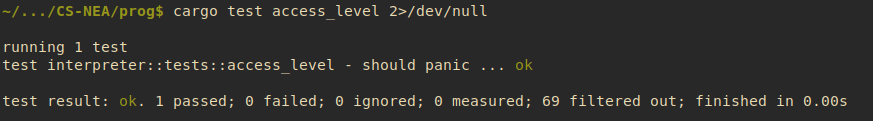
\includegraphics[width=\textwidth]{after_access_level}
	\caption{Screenshot showing the access modifier test succeeding}
	\label{lst:after_access_level}
\end{figure}

\subsection{Stage \subsecnum}

For stage \subsecnum, we added tests that make use of the \texttt{input()}
function. The way they work is that they attempt to read from the corresponding
\texttt{.stdin} file and if it succeeds uses that as the input to the program.
\autoref{fig:do_until1} shows a test using the \texttt{input()} function
passing.

\begin{figure}
	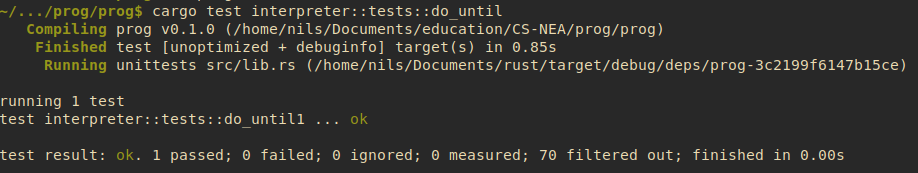
\includegraphics[width=\textwidth]{do_until1}
	\caption{Screenshot of a test using the \texttt{input()} function passing}
	\label{fig:do_until1}
\end{figure}

\subsection{Stage \subsecnum}

When playing around with the playground, we noticed an issue, the worker seemed
to be unresponsive after too many errors occurring. We decided to fix it by
restarting the worker whenever an error occurs and by disabling the action
buttons on the playground until the worker is ready to accept code. This fixed
the issue entirely and the playground now works perfectly even when panics
occur.

We suspect the module wasn't usable after panics because the memory was
corrupted as rust programs are not meant to continue working after a panic.

\subsection{Stage \subsecnum}

Whilst testing our interpreter against some of the examples offered by
\citetitle{pseudocode-uk} we found that examples which defined a global array
were not parsed correctly. This can be seen in
\autoref{fig:global_array_declaration_failing}.

\begin{figure}
	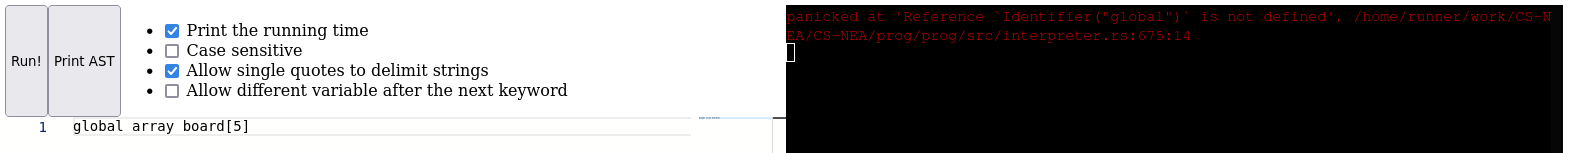
\includegraphics[width=\textwidth]{global_array_declaration_failing_run}
	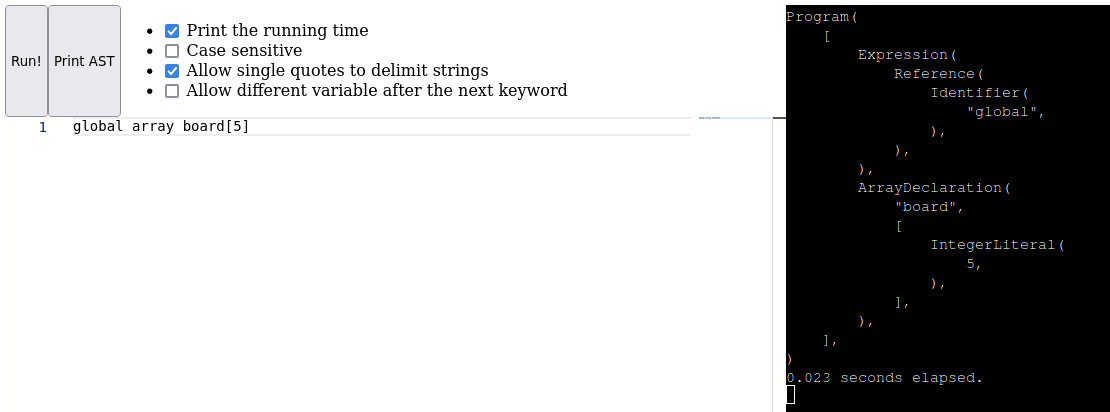
\includegraphics[width=\textwidth]{global_array_declaration_failing_ast}
	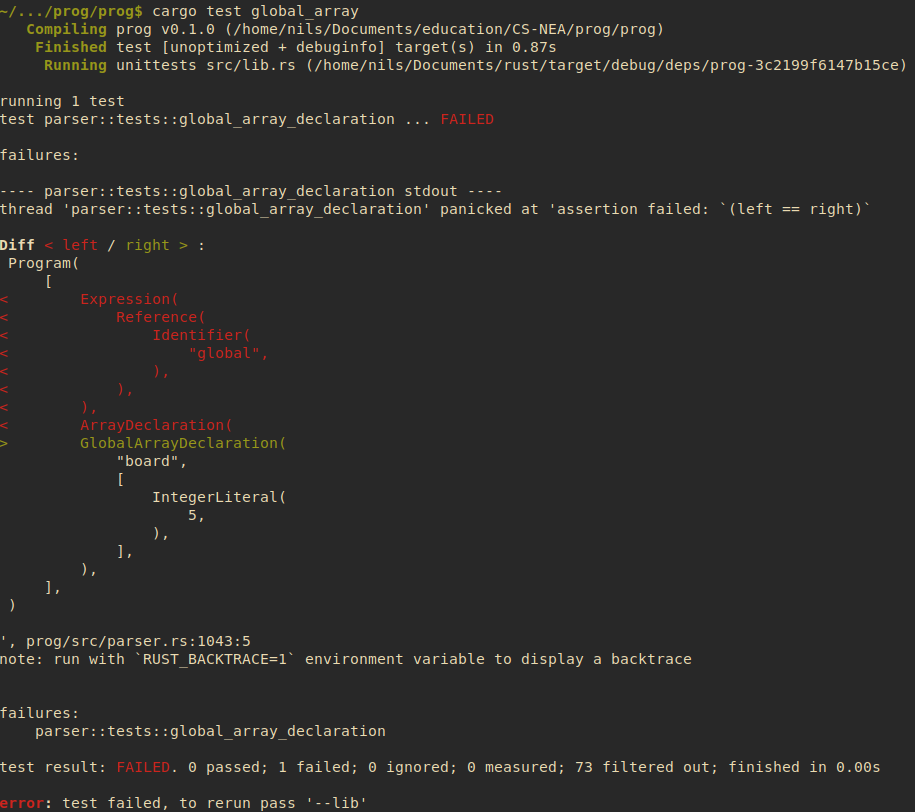
\includegraphics[width=\textwidth]{global_array_declaration_failing_test}
	\caption{Three screenshots demonstrating that global array declarations do
	not work}
	\label{fig:global_array_declaration_failing}
\end{figure}

We have decided to fix this by adding a new variant to the Statement object,
\texttt{GlobalArrayDeclaration} which is identical to
\texttt{ArrayDeclaration} instead of a common type between the two. The reason
behind this is that writing a common type between the two would require
changing all  the \texttt{.ast} files that make use of array declarations, an
operation that is time consuming.

\begin{figure}
	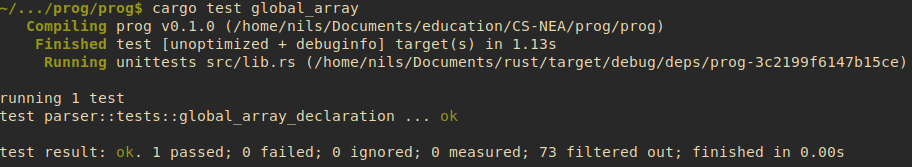
\includegraphics[width=\textwidth]{global_array_declaration_success_test}
	\caption{Screenshot of test for global array declaration passing}
	\label{fig:global_array_declaration_success}
\end{figure}

After the fix was implemented \autoref{fig:global_array_declaration_success}
demonstrates that the fix worked and was effective.

\subsection{Stage \subsecnum}

For this stage we wanted to test our programming language further and to do so,
we wrote a small program which calculates the roots of a quadratic equation.

\begin{listing}
	\inputminted{text}{./code_examples/quadratic_solver.prog}
	\caption{Source code for the quadratic equation solver}
	\label{lst:quadratic_solver}
\end{listing}

However, it did not run successfully because of some unimplemented features in
the language as can be seen in \autoref{fig:quadratic_solver}. Becaues of this
we decided to add it as a test to our test suite and implement the features
required.

\begin{figure}
	\begin{minted}{text}
% prog-cli ./code_examples/quadratic_solver.prog
Enter the first coefficient: 1
Enter the second coefficient: -3
Enter the third coefficient: -10
thread 'main' panicked at 'Reference `Identifier("-b")` is not defined', prog/src/interpreter.rs:677:14
note: run with `RUST_BACKTRACE=1` environment variable to display a backtrace
	\end{minted}
	\caption{Ouput of running the quadratic solver}
	\label{fig:quadratic_solver}
\end{figure}

We can see from the error message that ``\texttt{-b}'' was recognised as its
own identifier instead of as the negative of b. This is because unary
operations have not been implemented in the language so we will implement them.

We decided to implement both unary plus and unary minus operations to be less
restrictive however not implementing unary plus is always a possibility. For
example \citetitle{rust} does not implement the unary plus operation leading to
a parsing error however python does support the operation.

\begin{figure}
	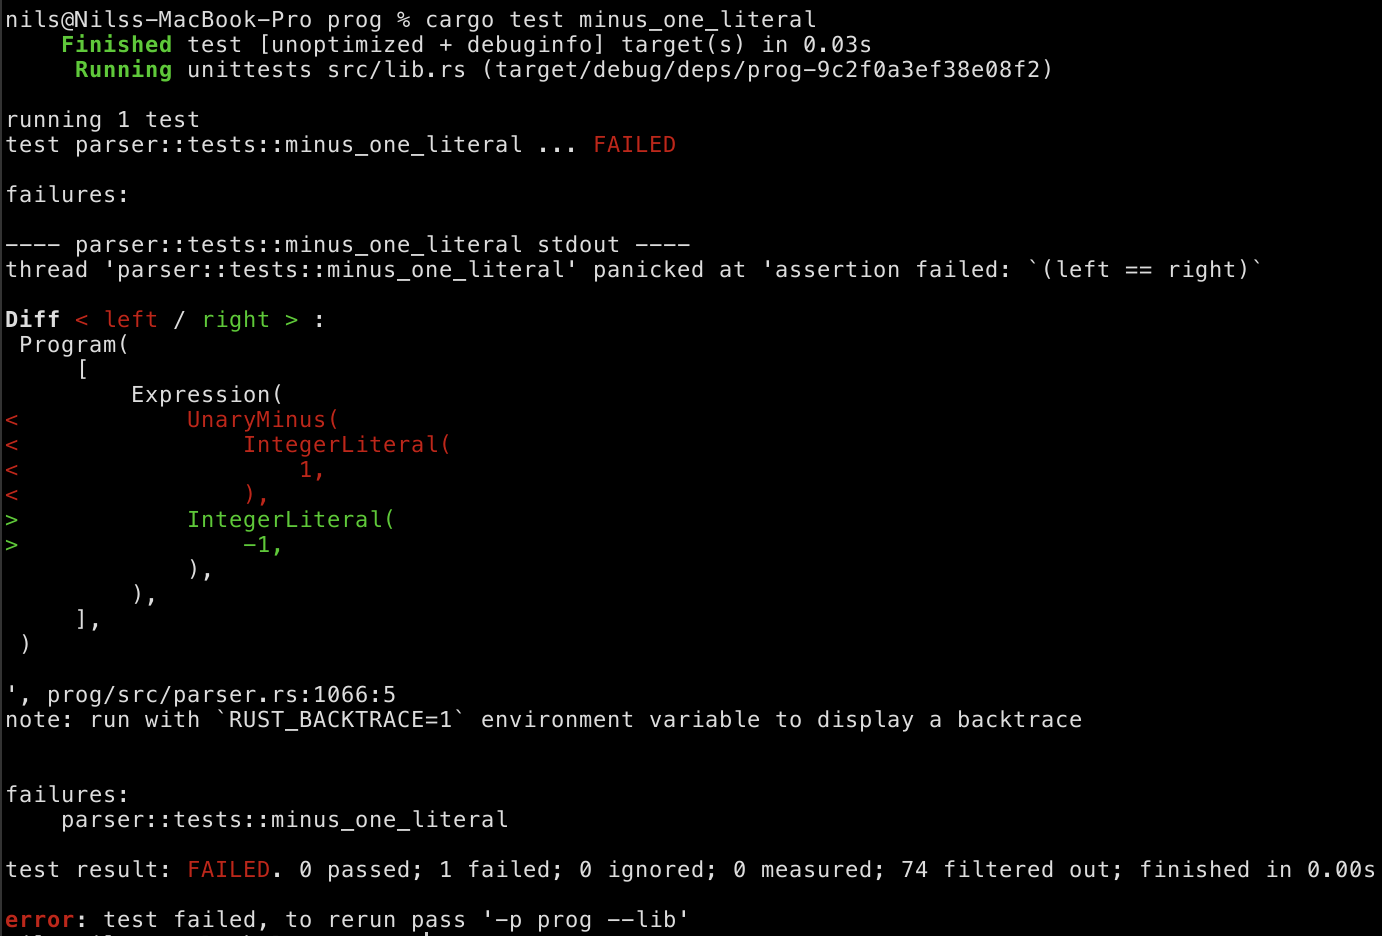
\includegraphics[width=\textwidth]{unary_minus_causes_regression}
	\caption{Screenshot of a test failing after adding the unary minus operator}
	\label{fig:unary_minus_causes_regression}
\end{figure}

However this caused another test to regress as can be seen in
\autoref{fig:unary_minus_causes_regression}. This is a test we added in an
earlier stage when we couldn't parse negative numbers. However the solution we
implemented at the time is inadequate and this one is more appropriate as it is
more general. To fix this failing test we will simply change the \texttt{.ast}
file to match the new output.

Now all the tests pass as can be seen in \autoref{fig:unary_minus_test_pass}.

\begin{figure}
	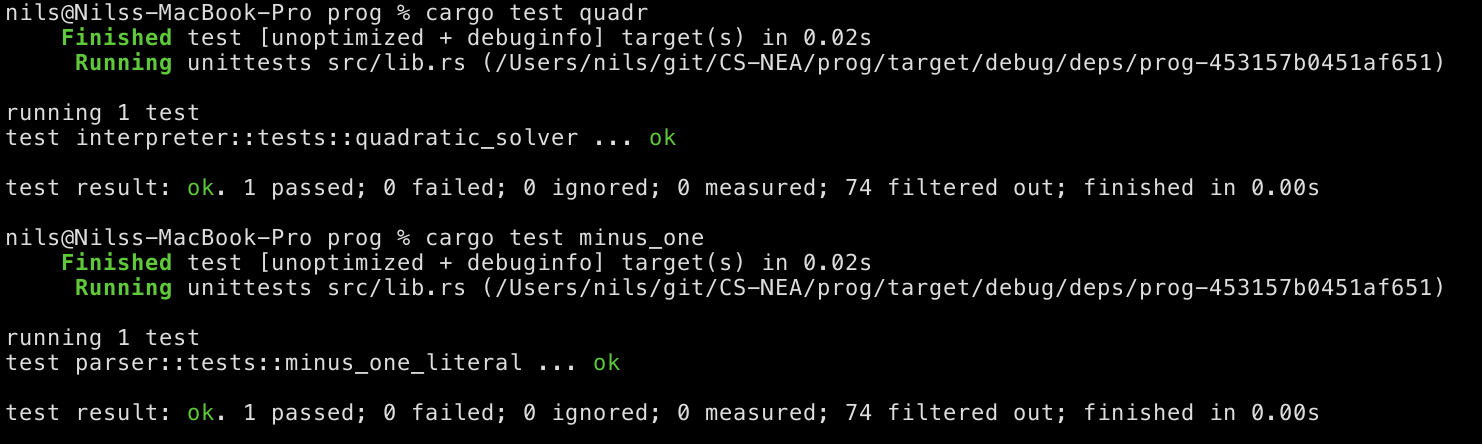
\includegraphics[width=\textwidth]{unary_minus_test_pass}
	\caption{Screenshot of tests passing after the changes are implemented}
	\label{fig:unary_minus_test_pass}
\end{figure}

\section{Evaluation}

% implement better cli with features
% differ from other pseudocode: no implicit cast, space in keywords, processes
% functions beforehand
% implement a way to share code in the playground
% look at the list of todos

% support files online is actually possible

\subsection{Testing and success criteria}

Because of our use of automated testing, every success criteria except for the
first (as visible in \autoref{tbl:success_criteria}) can be tested by running
the test suite (which includes all the tests mentioned in the success criteria
and more) which by now consists of more than 1000 lines of test code
distributed over more than 70 tests as can be seen in \autoref{fig:final_test}.

\begin{figure}
	\includegraphics[width=\textwidth]{final_test}
	\caption{Screenshot showing the full test suite passing}
	\label{fig:final_test}
\end{figure}

To test the first item of the success criteria, which is to execute a program
in a file from the command-line interface (CLI), we will write a program to
verify the correct solution for the OCR A level June 2018 paper, where the
binary tree algorithm is implemented. This example from the exam board uses
\texttt{null} values, something that we have not implemented because they
appeared nowhere in the specification. This is why we will first implement null
values (we consider any document from OCR to fully respect the rules of the
language).

Now we had to implement some of the functions used by the code example such as
the Node class used in the binary tree. \autoref{fig:2018_Q1c} shows the result
of running the code and the code used is the following:

%\begin{listing}
\inputminted{text}{./code_examples/2018_Q1c.prog}
%	\caption{Source code to test out function written in the mark scheme}
%	\label{lst:2018_Q1c}
%\end{listing}

\begin{figure}
	\includegraphics[width=\textwidth]{2018_Q1c}
	\caption{Screenshot of terminal when testing the program}
	\label{fig:2018_Q1c}
\end{figure}

We also tested a queue program which worked as intended as can be seen in
\autoref{fig:queue}. The code of the program follows:

\inputminted{text}{./code_examples/queue.prog}

\begin{figure}
	\includegraphics[width=\textwidth]{queue}
	\caption{Screenshot of queue program working}
	\label{fig:queue}
\end{figure}

We believe that some of the decisions that were taken such as the one to use
rust's testing framework instead of writing our own testing tool was a very
positive decision. Not only did it save time as nothing additional had to be
written it also means that testing can be automated much more easily and we
benefit from the large ecosystem of rust including, if we wanted to with the
ability to view how much of our code is covered by tests (code coverage).

Looking at the examples of code from \textcite{pseudocode-uk} most of them
didn't run on our interpreter for various reasons. One of them is that if a
call to a function that was defined later was done, the code would work and
still code a function defined later. In our interpreter, this is not possible,
functions and classes must be declared before they are called. We believe that
this behaviour is acceptable because it is the behaviour of python and the
language is a very dynamic one so most users would not expect the language to
support references to items defined later in the code. Another thing that is
featured in these examples is the use of a space between ``end'' and another
keyword like ``function''. This is something that is not defined in the OCR
Reference Language and as such we have not implemented it, we do not believe it
is correct.

\subsection{Unmet criteria}

There are no unmet criteria for the main project. The interpreter from the
command line interface is fully functional and supports all the features of the
OCR Reference Language and more.

However, whilst developing the project we realised it would be very hard to use
a CLI for most people so we developed a playground to test out the language.
This playground is fully functional and supports all the features of the
language except the ones that do not make sense on the web, such as file
operations and the \texttt{system} function. However a function that was
originally planned was the use of the \texttt{input()} function to accept input
from the user. Unfortunately this function does not work on the playground
because of JavaScript's and the web's asynchronous nature. It is not possible
for our synchronous web assembly module to wait for input from the user as that
would necessarily require our program to work asynchronously. In order to fix
this issue, there are two ways that we can think of. Firstly, convert our
program to be asynchronous. This is an option that is possible as rust's Future
is compatible with JavaScript Promises, the types that represent something that
has not yet been computed in the respective languages. However it would mean
rewriting large portions of our interpreter and adding dependencies to
asynchronous runtimes, all of that for something that already works for the CLI
interface. Another solution would be to use a channel between the worker and the
web page that is synchronous. This is possible with the
\texttt{SharedArrayBuffer} type in combination with the \texttt{Atomics} module
of the JavaScript API. There are also packages such as
\citetitle{shared_channel} which implement the channel already, although because
of the way \citetitle{shared_channel} is implemented, it would require creating
a new crate in our project which both the WebAssembly module and the web page
would depend on to communicate using a common language. However because of the
use of the \texttt{SharedArrayBuffer} this would require setting certain HTTP
response headers from the server for security purposes\footnote{These
requirements were introduced in light of the Spectre vulnerabilities} which
would mean changing hosting provider as as of the time of writing GitHub Pages
don't support setting HTTP headers. However there are alternatives to GitHub
Pages like Cloudflare Pages which support headers at no additional cost so this
doesn't defeat the economic advantage of having a static website\footnote{After
completion of the NEA, we implemented input on the playground which meant
having to change the hosting provider so the playground linked is actually
hosted on Cloudflare Pages and does support \texttt{input()}}.

In regards to additional features we had envisioned for the language and to
make it more usable, we have implemented only the playground. Considering the
playground has been built we believe that most users will use that instead of
the CLI interface for most of their usage, this means that implementing syntax
highlighting for the playground alone would be a worthwhile investment as it
would benefit a majority of the userbase. Additionally because the monaco
editor is used by Visual Studio Code, a syntax definition for monaco would be
compatible with Visual Studio Code. Which means that users of the most popular
text editor since 2018 will also benefit. We however do not believe that
implementing a language server for the language would be worth it. It would be
a significant effort when improving the error messages itself would benefit far
more.

We have however not implemented any of the optional features on the
command-line interface. This means that if a user wants to use some of the
optional language feature/settings on the command line they will be unable to
and will have to use the playground which itself has some other missing
features (e.g. file system support and input). However we believe that
implementing features to the command line would be quite trivial as we are
already using the clap argument parser which means only a few lines of code
would be required.

\subsection{Maintenance and limitations}

One major maintenance issue that our programming language has is its parser.
Because we wrote a parser manually we spent a long period of time on this
section of the project when using a parser generator would have done the job a
lot better and made the parser more maintainable. As it stands, changes to
parsing require modifying the parser, something that is error prone, if a
parser generator had been used, it would only require changing a declarative
grammar that is a lot easier to understand. This difficulty of maintenance
ultimately increases the number of bugs and also had a negative impact on
performance as corners are cut\footnote{In rust, a lot of borrow checker issues
can be fixed by cloning values instead of passing references to them. Cloning a
value is an expensive operation which requires memory allocation and ultimately
results in decreased performance.}. In particular when implementing
precedence we have to write very nested and difficult to read code, something
that would have been avoided had a parser generator been used instead. Overall
durring the development many bugs occured in the parser and it is a section
that is difficult to debug due to its terrible error making the maintenance
even more difficult.

Another major maintenance issue with the parser is its testing. When testing
it, abstract syntax tree produced is compared to an abstract syntax tree loaded
from a file. This causes a big issue whenever the structure of the tree is
modified resulting in the files containing abstract syntax trees having to be
modified. This meant that multiple times during development, because of a
small change in the structure of our abstract syntax tree, we had to modify a dozen files
to be able to make tests work again. This could be fixed in different ways, one of
them is to write migration code, similarly to migrations in databases, which
convert these files into the new format whenever a change happens. Another way
would be to use the output of our parser to write these files, without having
to write them manually beforehand. This is possible with packages such as
\citetitle{insta} which automatically do all the heavy-lifting for us. This
library will automatically write files to the appropriate place and update them
when the test result changes, first asking the developer if the change should
be accepted or not. A downside of this method is that there is a risk of bias,
as the intended test results are determined based on the output of the current
program rather than from a human which doesn't have the same bugs as the
program could have. This method is however faster and easier to implement than
having to migrate files using code (rather than automatically).

Although our testing is quite thorough, it could be much better. In particular
we have currently no way of knowing how much of our code is actually being
tested. In order to know that, we would need to find out our code coverage, how
much of a our code is covered by tests. Considering we are using rust's
built-in testing framework, it is very easy to add support for code coverage,
although we didn't take the time to support it as part of our allotted
development time. By having code coverage, it will be possible to determine
which parts of the codebase are not tested which then makes it possible to
write additional tests to cover this forgotten areas, furthermore code coverage
can give us an estimation of how thorough our testing is, to have a measure of
how likely an uncaught bug could occur. Do note however, that code coverage is
not necessarily associated with decreased number of bugs, low quality testing,
can still let a lot of bugs appear even with a large code coverage.

Another testing method we could make use of is fuzzing. It consists of having
another program, the fuzzer, automatically test our software. This method is
one of the main way that memory corruption vulnerabilities are found nowadays
as it is a very difficult task now that mitigations have removed a large amount
of memory corruption bugs. Because our programming language is written in a
memory safe programming language, memory corruption related bugs are very
unlikely to happen however they could if an erroneous use of the
\texttt{unsafe} keyword\footnote{In rust, the \texttt{unsafe} keyword is used
to disable some of the checks made by the compiler which normally would
guarantee memory safety, it is up to the programmer to make those guarantees.
This keyword allows to write certain things which would normally not be
possible at the risk of there being a memory corruption bug occurring.} is used
in one of our dependencies. The reason fuzzing is good at finding memory
corruption vulnerabilities is because memory corruption bugs are the only
things it can find as it has no indication of what is valid or wrong behaviour,
it just tries to vary its input to cover the maximum amount of the software,
detecting an error when the program aborts, something that mainly happens due
to memory corruption bugs.

Another type of test that could have been carried out more thoroughly is
benchmarks, they allow to measure the performance of our implementation of the
programming language and compare it to others. Although our language is not
designed to have a great performance high performance is beneficial and makes
the language more usable. We have however performed limited benchmarks by
writing a program to calculate the largest prime smaller than 100'000 in three
different languages visible at \autoref{tab:bench_prime}. This simple benchmark
is however quite interesting and shows that our language is about twice as slow
as python, which is notoriously slow.

\begin{table}
	\begin{center}
		\begin{tabular}{|c|l|S|}
			\hline
			Language & Runtime & {Time (s)} \\
			\hline
			OCR Reference Language & Web Assembly & 198.331 \\
			\cline{2-3}
			listing \ref{lst:bench.prog} & Native & 102.902 \\
			\hline
			Python & CPython & 54.422 \\
			\cline{2-3}
			listing \ref{lst:bench.py} & PyPy & 8.450 \\
			\hline
			Rust & No optimisations & 8.422 \\
			\cline{2-3}
			listing \ref{lst:bench.rs} & \texttt{opt-level=3} & 1.044 \\
			\hline
		\end{tabular}
	\end{center}
	\caption{Results of prime number calculation benchmark}
	\label{tab:bench_prime}
\end{table}

\begin{listing}
	\inputminted{text}{./code_examples/prime.prog}
	\caption{Prime number benchmark in OCR Reference Language}
	\label{lst:bench.prog}
\end{listing}

\begin{listing}
	\inputminted{python}{./code_examples/prime.py}
	\caption{Prime number benchmark in python}
	\label{lst:bench.py}
\end{listing}

\begin{listing}
	\inputminted{rust}{./code_examples/prime.rs}
	\caption{Prime number benchmark in rust}
	\label{lst:bench.rs}
\end{listing}

One of the reasons that our language is slow is our heavy use of hash tables to
store variables this means that every access to a variable is a costly
operation. In the future an improvement that could be made to the language is
to use lexical addressing, a method in which variables are turned into indices
in an array, thereby greatly improving performance.

A major limitation of the current implementation is the almost unreadable error
messages, although they have been improved with the interpreter in
\hyperref[sec:better_errors]{Stage 24}, trying to understand where a syntax
error is located is a difficult challenge which even someone with an idea of the
internals of the parser has trouble understanding.  This issue could be fixed in
many ways, part of the issue is that data about the initial source code is
discarded after it is parsed and as such it is not possible to display to the
user which line of code caused a runtime error. A solution would be to include
this data in the abstract syntax tree. Error messages could also be improved by
using the tooling that nom provides to make better error messages. However both
of these solutions would be quite complex to implement and as such it may be
preferable to start by using a parser generator which would make most of these
issues much easier to handle. We had originally planned to use tree-sitter as
our parser, so it may be the opportunity to go back to tree-sitter and use it as
our parser. In the current version of the playground, the editor used is the
monaco-editor which doesn't support tree-sitter yet, but instead uses its own
syntax definition format. This means that the benefits of using tree-sitter
would be reduced as we wouldn't be able to use it for syntax highlighting,
nevertheless, implementing tree-sitter has further benefits such as the
potential it has for writing further tooling such as linters\footnote{A linter
is a static code analysis tool that flags programming errors, bugs, stylistic
errors and suspicious constructs}\cite{ben_tree_sitter_linter}.

Still in regards to errors, we currently only have two tests that check a
program fails to run and both tests are written manually instead of using a
macro like we usually do. This means that adding more tests in the future will
be error prone and time consuming, so to make the interpreter more
maintainable, declaring tests that should fail should be done using a macro.
Additionally, these tests to done restrain what type of error should occur
which means that if the program fails to execute for a reason other than the
reason it should, it will not be detected. In order to fix this, we would have
to improve the error system so that errors are returned based on what failed to
execute and which means we should stop the use of panic to communicate error
message to the user, something that is heavily discouraged. Panicking in rust
should only be used for errors that are unpredicted or unrecoverable from which
aren't the case for most errors that a user will encounter.

To make the programming language more usable, having a REPL\footnote{A
read-eval-print loop (REPL) is an interface in which the user types commands and
gets the results of the operation back} would be nice. A REPL would allow users
to quickly develop their programs and trying out the different features the
language provides without having to run everything from scratch. A REPL could
also be used to then build a debugger where once a break point is reached the
user can type commands as if they were in the language.

Additionally currently there are no settings for the interpreter, only some for
the parser. This means that additional features we added in the interpter such
as the system function aren't behind a flag/setting and are always enabled. It
would be beneficial to add support for these settings something that can be
done by adding settings within the \texttt{Context} struct, an object that is
alive for the entire duration of the interpreter.

Although not of great interest considering the use case of the language, an
evolutionary step that could be taken would be the implement a compiler for the
language in the language itself. If this is successful it would allow the
language to be self hosted and extremely performant.

A usability feature that could be added to the playground is the ability is
share code, this is something that playgrounds in most programming language
support. Sharing code would allow teachers to rapidly show a snippet of code to
their students or for a student to share some code quickly. There are two ways
this could be implemented, either as a parameter in the URL that contains the
entire code snippet or as stored code on the server. The advantage of storing
the code on the server side is that it allows to share short URLs however it
means that a back-end needs to be implemented to store the code. Alternatively,
an already back-end could be used such as one of the ones used by many of the
already existing ``pastebin'' services. The second method is to store the code
within the URL with a query parameter or using the fragment identifier. These
methods are less complex to implement as they don't require a backend but they
mean that the entirety of the shared code is within the URL which can get very
large. Certain web servers and browsers have a limit on the length of the URL
which would cause issues with this method. A hybrid approach can always be
considered.

Another feature to make the playground more user-friendly would be to have
example programs users can load to test out the playground. For the moment the
only example program we have is a hello world program which cannot be changed
for something else.

Although file operations on the web do not work and are not intended to work,
it would actually be possible to implement them through a virtual file system,
a file system that exists within the web page. This approach is the one used by
\citetitle{emscripten}\footnote{a C/C++ compiler to WebAssembly which also
supports any language which compiles to LLVM}. It would also be possible to
support file system operations through the use of the Native File Access API, a
new API which allows to access the local files of a user after they have given
their permission.

\section{Conclusion}

For this project, we have demonstrated the need for the ability to be able to
execute programs written using the OCR Reference Language (also known as the
OCR pseudocode in older specifications such as the A-level one).

Our developed project has a modular structure made up of the back-end. A parser
and interpreter for the programming language. And it features, two front-ends,
a command-line interface downloadable from
\url{https://prog.tools.nilsand.re/prog-cli.exe} and a web interface developed
using the help of Web Assembly available at
\url{https://prog.tools.nilsand.re/}.

Although they are still minor bugs in the software we consider our project
mainly completed to a very high standard of development and with very low
technical depth thanks to a very rigorous use of automated testing and
following the best practices used in software engineering. We also attribute
the correctness of our implementation to the strong typing of Rust which has
allowed us to restrict our software by the use of the type system to improve
its correctness.

Outside of the scope of this report we plan to polish the software for it to be
usable for the students that will study Computer Science at A-level and GCSE
for the coming years.

\section{Final project}
\label{sec:final_project}

This section lists our final code as well as describe the structure of the
project for someone interested in running it.

\subsection{Dependencies}

In order to compile the final project, here is a list of dependencies:

% FIXME: do we actually need rust nightly?
\begin{itemize}
	\item Rust (nightly)
	\item Node.js (for playground)
	\item wasm-pack (for playground)
\end{itemize}

A pre-compiled binary for windows is available at
\url{https://prog.tools.nilsand.re/prog-cli.exe}.

\subsection{Running / Structure of the files}

After un-archiving the files, one is faced with a few directories. The
\texttt{prog} directory contains the back-end/library for the language.
\texttt{prog-cli} contains the command-line interface, just a few lines of code
calling the library. \texttt{www} contains the playground. \texttt{prog-wasm}
contains the rust code to make it work in the playground.

To run the command line interface, just run \texttt{cargo run} anywhere in the
project. Use \texttt{cargo run -- --help} to view the help menu. The
command-line interface just accepts a file as its first argument which it will
execute. It can also execute a program from standard input if no file is given.

To run the web interface go to the \texttt{www} directory and run \texttt{npm i
\&\& npm run serve}. To build the website into the \texttt{dist} directory run
\texttt{npm i \&\& npx webpack}.

\subsection{Download}

Some of the listings in the following section are not displayed correctly. For
example, some lines are too long and go over the page and some of the
characters, in particularly the chess pieces and the curved double quotation
marks are not displayed correctly. To be able to navigate the project, without
these mistakes, here are 2 attachments of it in
\textattachfile{./final_files.zip}{zip} and
\textattachfile{./final_files.tar.gz}{tar.gz} format (some PDF viewer do not
support attachments, Firefox and Adobe Acrobat Reader are known to work,
macOS's Preview and Google Chrome \textbf{do not} work).

\subsection{Listing}

\newgeometry{margin=1in}

\input{./final_files.tex}

\printbibliography[heading=bibintoc]

\end{document}
